\documentclass[11pt,a4paper]{article}
\usepackage[margin=2.2cm]{geometry}
\usepackage[T1]{fontenc}
\usepackage{lmodern}
\usepackage{graphicx}
\usepackage{amsmath}
\usepackage{amssymb}
\usepackage{booktabs}
\usepackage{tabularx}
\usepackage{array}
\usepackage{float}
\usepackage{placeins}
\usepackage{xcolor}
\usepackage{underscore}
\usepackage{hyperref}

\hypersetup{hidelinks,
pdftitle={CS683 PA2: Prefetching and Instruction-Conscious Replacement},
pdfauthor={Balaji, Kamyak, Harith, Aayush}}
\setlength{\parindent}{0pt}
\setlength{\parskip}{5pt}
\setlength{\emergencystretch}{2em}

% Each task restarts section, table and figure numbering, as in the
% original separate reports (Task 3's text refers to "Table 2").
\counterwithin*{section}{part}
\counterwithin*{table}{part}
\counterwithin*{figure}{part}
\counterwithin*{equation}{part}
\renewcommand{\theHsection}{\thepart.\arabic{section}}
\renewcommand{\theHtable}{\thepart.\arabic{table}}
\renewcommand{\theHfigure}{\thepart.\arabic{figure}}
\renewcommand{\theHequation}{\thepart.\arabic{equation}}

\title{\textbf{CS683: Advanced Computer Architecture (PA2)}}
\author{Balaji (23B1029), Kamyak (23B0949)\\
Harith (23B1085), Aayush (23B0944)}
\date{15 October 2026}

\begin{document}
\maketitle

\tableofcontents

\clearpage
\part{Task 1: L1D Data Prefetching}

 Task 1a describes the IP-stride prefetcher
provided with ChampSim. Task 1b implements a Stride Pattern Prefetcher
(SPP) at L1D that learns repeating, possibly non-uniform, stride
sequences per IP, and compares it with IP stride and no prefetching on
the three traces.


\section{Task 1a : IP Stride}

The IP stride uses a tracker to store the IP index, the last address
accessed by the IP, the last stride, and the LRU index of the entry.
There are 24 trackers. The IP is masked with \texttt{0xFF}, so the code
only uses its last 8 bits to find the tracker. Two different IPs can
therefore end up using the same entry.

When there is a memory access from the IP, the code converts the address
to a cache-line address and finds the difference from the previous
address. This difference is the stride. If it is the same as the last
stride, the prefetcher issues requests with a fixed degree of 3.
It needs two equal nonzero strides before it starts prefetching.

For example, if the accessed cache lines are 100, 102, and 104, the two
strides are both 2. At 104, the prefetcher requests 106, 108, and 110.
The strides are in cache lines, not bytes. A cache line is 64 bytes.
Negative strides work in the same way. The requests start at the next
predicted access, so the distance is fixed at one predicted access.

After this, IP stride updates the last address and stride for the next
access. For a new IP, it removes the least recently used tracker, saves
the current address, and returns without prefetching. The LRU counter
is used to choose the tracker to replace.

Every request is checked against the current 4 KB page. Prefetching
stops if the next address crosses the page boundary. If the L1D MSHR
occupancy is below half its size, the request is sent to L1. Otherwise,
it is sent to L2. An access to the same cache line has stride zero and
returns immediately.

This works well for a constant stride. It cannot learn the whole
sequence when the strides keep changing, such as \texttt{[1,2,2,2,3]}.

\section{Task 1b: Stride Pattern Prefetcher}

My idea for the Stride Pattern Prefetcher is to store an array of
strides accessed till now, separately for each IP. If the pattern seems
to repeat, I increment the \texttt{num\_iterations} counter and keep
continuing the array access. This lets me represent both uniform and
non-uniform strides using the same array.

A uniform stream can have a single element stride array. A repeating
non-uniform stream can have several elements, such as
\texttt{[1,2,2,2,3]}.

\subsection{Updating the stride array}

If the \texttt{stride\_array} had \texttt{[1]} and the
\texttt{num\_iterations} was 2, then a new stride of 2 would make the
array \texttt{[1,1,1,2]}. The first 1 was already in the array. The next
two came from the matches counted by \texttt{num\_iterations}.

The \texttt{curr\_index} tells me which stride is expected next.
On a match, it advances and wraps around at the end of the array.
The iteration counter is increased at index zero, so it counts the
cycles that have started. If a mismatch happens partway through a
cycle, I keep the completed cycles and the matched part of the current
cycle before adding the new stride.

I limited the array to 16 strides. Before expanding it, I check how
many entries are needed. If it would exceed 16, I restart the array
with the current stride. This loses the old pattern, but it keeps the
storage fixed and avoids writing outside the array. The iteration
counter is also capped at 16.

\subsection{Uniform and non-uniform predictions}

For dynamic checking of both uniform and non-uniform accesses, I made
the prefetcher check both cases. There is one confidence counter for
uniform strides and another for the array pattern. Both are bounded
by \texttt{MAX\_CONFIDENCE = 3}.

The uniform counter increases if the stride is the same as
\texttt{last\_stride}. Otherwise, it becomes zero. Uniform prediction
starts when this counter is at least 1. This means two consecutive
strides were equal, just like the check in IP stride.

The non-uniform counter increases when the current stride matches the
expected array element. It becomes zero on a mismatch. The next
prefetch addresses are formed by adding the following array elements
one by one. For example, after matching the first 1 in
\texttt{[1,2,2,2,3]}, four predictions add 2, 2, 2, and 3 to the address
in that order.

The uniform requests are issued first. The current code also issues
array predictions on the same access if the array matches. Each
predictor has its own degree, so both can issue requests together.
This can produce duplicate requests, especially for a one-element
array. The simulator may merge them later.

\subsection{Degree based on confidence and accuracy}

For each predictor, I use
\[
\text{degree} = \min(3 + \text{confidence},\;\text{accuracy degree limit}).
\]
The base degree is 3. A confident predictor can go up to 6, while the
accuracy limit can bring it back down to 3. Since the two predictors
have separate budgets, the code can attempt up to 12 requests on one
access. The limit of 6 is per predictor, not a combined limit.

ChampSim already updates \texttt{pf\_useful} when a prefetched line is
used, and \texttt{pf\_useless} when an unused prefetched line is evicted.
I use these counters to calculate accuracy over recent outcomes. After
at least 128 new outcomes, I calculate
\[
\text{feedback accuracy} =
\frac{\Delta\texttt{pf\_useful}}
{\Delta\texttt{pf\_useful} + \Delta\texttt{pf\_useless}}.
\]

\begin{center}
\begin{tabular}{lll}
\toprule
Recent accuracy & Change in degree limit & Bound \\
\midrule
Below 25\% & Decrease by 1 & Minimum 3 \\
25\% to 50\% & Keep the same limit & No change \\
Above 50\% & Increase by 1 & Maximum 6 \\
\bottomrule
\end{tabular}
\end{center}

The limit starts at 6. The middle range avoids changing it after every
small fluctuation. Updating after 128 outcomes also avoids making a
decision from just one useful or unused prefetch. These values were
chosen for this implementation and tested with the traces; they are
not fixed values taken from a paper.

ChampSim resets its counters after warmup. I check for this reset and
update the saved counter values before subtracting them. Otherwise,
unsigned subtraction could give a very large value and make the
accuracy calculation wrong.

All predictions still use the same-page check and the L1/L2 fill rule
from IP stride.

\subsection{Metrics used}

IPC is the number of retired instructions divided by the cycle count.
Speedup is the prefetcher IPC divided by the no-prefetch IPC.
L1D load MPKI is the number of demand-load misses per 1,000 instructions.
Coverage is calculated as
\[
\text{coverage} =
\frac{\text{baseline load misses} - \text{prefetcher load misses}}
{\text{baseline load misses}}.
\]

For the accuracy in the result tables, I used the value printed by
ChampSim. In this version of the simulator, it is
\[
\text{reported accuracy} =
\frac{\text{useful prefetches}}{\text{prefetch requests sent to a lower level}}.
\]
This is different from the recent useful/unused ratio used to control
degree. Also, \texttt{pf\_issued} can include requests that merge or
hit an existing line, so it is not the same denominator. There is no
accuracy value for the no-prefetch baseline.

\section{Results}

The SPP results below use the current raw stride-array code, with both
confidence counters and accuracy-based degree control. The latest
control rerun matched the earlier final results exactly on all three
traces, including cycles and prefetch counts.

\begin{table}[htbp]
\centering
\small
\setlength{\tabcolsep}{4pt}
\begin{tabular}{llrrrrr}
\toprule
Trace & Prefetcher & IPC & Speedup & Load MPKI & Accuracy & Coverage \\
\midrule
1 & No prefetch & 0.232204 & 1.000000 & 10.67872 & -- & 0.00\% \\
1 & IP stride & 0.233398 & 1.005140 & 10.11880 & 52.79\% & 5.24\% \\
1 & SPP & 0.233511 & 1.005631 & 9.92076 & 48.62\% & 7.10\% \\
\midrule
2 & No prefetch & 0.251130 & 1.000000 & 13.53380 & -- & 0.00\% \\
2 & IP stride & 0.251186 & 1.000225 & 13.43564 & 38.13\% & 0.73\% \\
2 & SPP & 0.251133 & 1.000011 & 13.43100 & 35.69\% & 0.76\% \\
\midrule
3 & No prefetch & 0.382061 & 1.000000 & 3.40324 & -- & 0.00\% \\
3 & IP stride & 0.382962 & 1.002359 & 3.31768 & 16.09\% & 2.51\% \\
3 & SPP & 0.383744 & 1.004404 & 3.20820 & 22.39\% & 5.73\% \\
\bottomrule
\end{tabular}
\caption{Results after 25M warmup and 25M simulation instructions.}
\end{table}

SPP has better IPC than IP stride on traces 1 and 3. IP stride is
slightly better on trace 2. SPP has fewer load misses and better
coverage on all three traces. Its accuracy is lower on traces 1 and 2,
but higher on trace 3. So the extra predictions help coverage, but
some of them are unused.

The geometric mean speedup over no prefetching is 1.003346 for SPP and
1.002573 for IP stride. This is about 0.335\% and 0.257\% respectively.
The gains are small, so I would not call any setting the best for all
programs based on these three traces.

\begin{figure}[htbp]
\centering
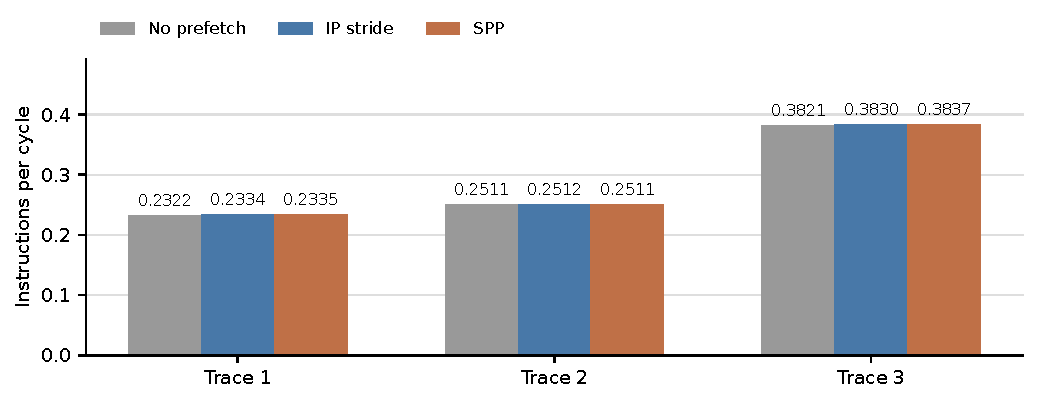
\includegraphics[width=0.92\linewidth]{figures/task1/ipc.pdf}
\caption{IPC of the baseline, IP stride, and SPP. Higher is better.}
\end{figure}

\begin{figure}[htbp]
\centering
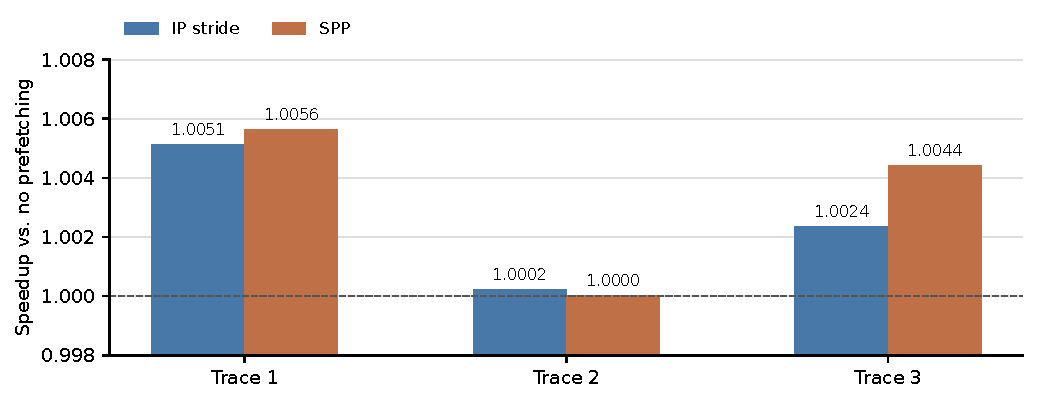
\includegraphics[width=0.92\linewidth]{figures/task1/speedup.pdf}
\caption{Speedup over no prefetching. The axis is zoomed around 1 to show the small differences.}
\end{figure}

\begin{figure}[htbp]
\centering
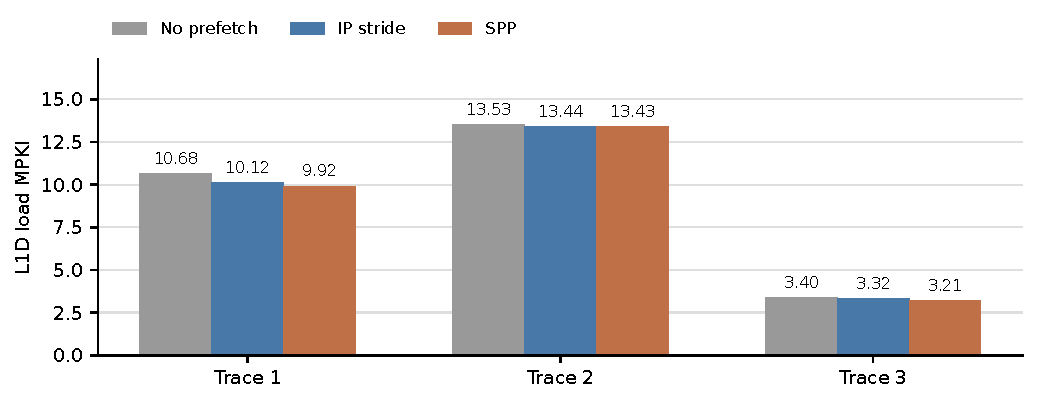
\includegraphics[width=0.92\linewidth]{figures/task1/mpki.pdf}
\caption{L1D load MPKI. Lower is better.}
\end{figure}

\begin{figure}[htbp]
\centering
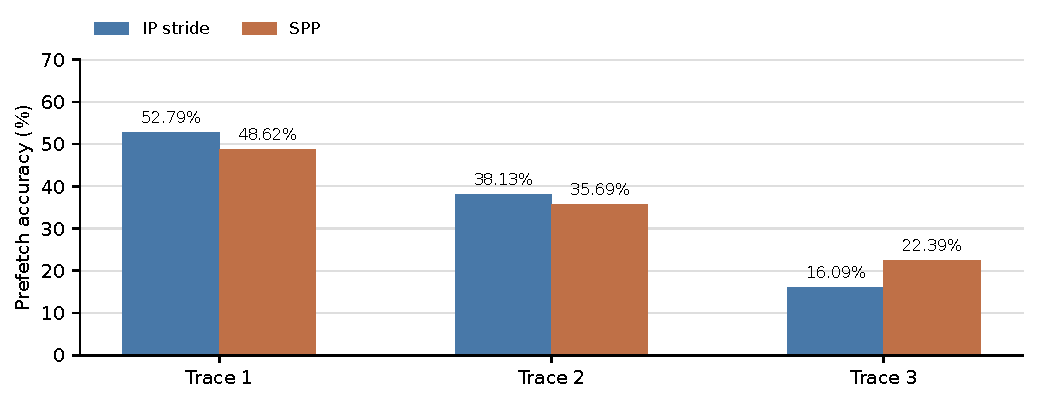
\includegraphics[width=0.92\linewidth]{figures/task1/accuracy.pdf}
\caption{Prefetch accuracy printed by ChampSim.}
\end{figure}

\begin{figure}[htbp]
\centering
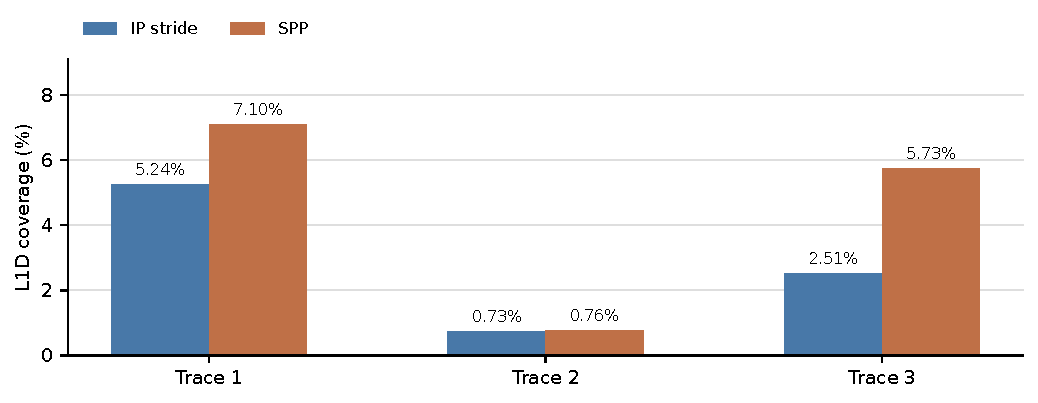
\includegraphics[width=0.92\linewidth]{figures/task1/coverage.pdf}
\caption{Coverage from the reduction in baseline load misses.}
\end{figure}
\FloatBarrier

\section{Other settings I tried}

\subsection{Fixed degree and confidence}

Before adding accuracy-based degree control, I tested fixed degrees of
3, 6, and 10. A higher degree did not improve IPC in these runs. It also
increased unused prefetches. This is why I kept 3 as the base degree
instead of always prefetching 6 or 10 lines.

\begin{table}[htbp]
\centering
\small
\begin{tabular}{rrrrr}
\toprule
Degree & Trace 1 IPC & Trace 2 IPC & Trace 3 IPC & Total unused \\
\midrule
3 & 0.233499 & 0.251192 & 0.383348 & 23,615 \\
6 & 0.233371 & 0.250855 & 0.383345 & 46,972 \\
10 & 0.233168 & 0.250662 & 0.382984 & 71,416 \\
\bottomrule
\end{tabular}
\caption{Fixed-degree tests using an earlier version of SPP.}
\end{table}

I also tried maximum confidence values of 1, 2, 3, and 5 with the earlier
fixed-degree version. In that version, uniform prediction waited until
the counter reached the maximum, and the array predictor was a fallback.
A value of 1 started uniform prediction sooner and gave better IPC on
traces 1 and 3. A value of 5 was slightly better on trace 2.

\begin{table}[htbp]
\centering
\small
\begin{tabular}{rrrr}
\toprule
Max confidence & Trace 1 IPC & Trace 2 IPC & Trace 3 IPC \\
\midrule
1 & 0.233605 & 0.251176 & 0.383646 \\
2 & 0.233515 & 0.251197 & 0.383372 \\
3 & 0.233499 & 0.251192 & 0.383348 \\
5 & 0.233475 & 0.251219 & 0.383312 \\
\bottomrule
\end{tabular}
\caption{Confidence tests using the earlier fixed-degree version.}
\end{table}

In the current code, I start uniform prediction at confidence 1 but
allow the counter to rise to 3. The extra confidence increases degree.
So the current use of maximum confidence is different from that earlier
test. The results above explain the changes I tried, but they are not
isolated comparisons against the final code.

\begin{figure}[htbp]
\centering
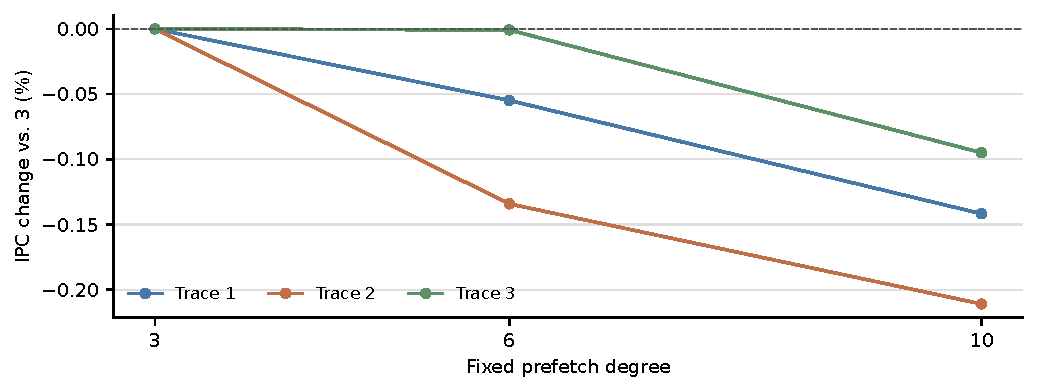
\includegraphics[width=0.92\linewidth]{figures/task1/degree_sensitivity.pdf}
\caption{IPC change from fixed degree 3 in the earlier degree tests.}
\end{figure}

\begin{figure}[htbp]
\centering
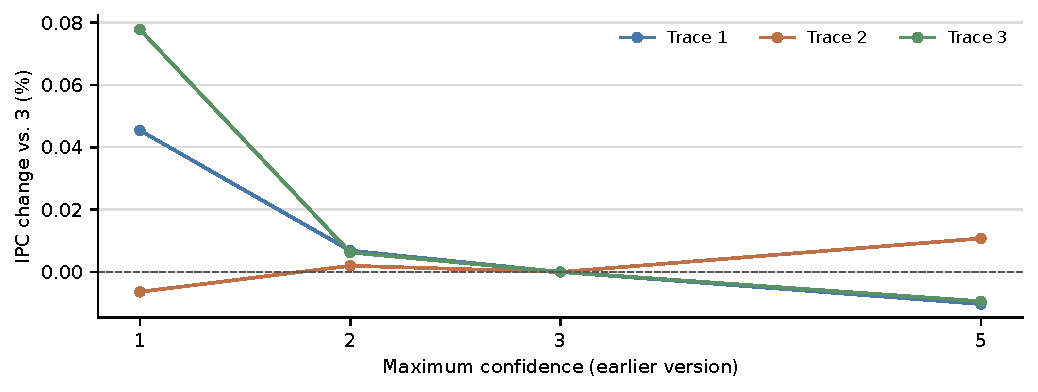
\includegraphics[width=0.92\linewidth]{figures/task1/confidence_sensitivity.pdf}
\caption{IPC change from maximum confidence 3 in the earlier confidence tests.}
\end{figure}
\FloatBarrier

\subsection{Choosing the accuracy settings}

I tested eight settings for the base degree, maximum confidence, uniform
activation, feedback window, and accuracy cutoffs. Each row below changed
one setting around the sweep control. That control had base degree 3,
maximum confidence 3, uniform activation at 2, a window of 128, and
25\%/50\% cutoffs.

\begin{table}[htbp]
\centering
\small
\begin{tabular}{lrr}
\toprule
Setting & Geometric mean gain over baseline & Total unused \\
\midrule
Uniform starts at 1 & 0.3421\% & 38,286 \\
Maximum confidence 2 & 0.3344\% & 31,403 \\
Window 64 & 0.3275\% & 32,335 \\
Sweep control & 0.3227\% & 32,816 \\
Cutoffs 35\% / 60\% & 0.3208\% & 31,168 \\
Base degree 2 & 0.3178\% & 24,931 \\
Maximum confidence 5 & 0.3164\% & 34,457 \\
Base degree 4 & 0.2987\% & 40,464 \\
\bottomrule
\end{tabular}
\caption{Earlier sweep of the confidence and accuracy settings.}
\end{table}

Uniform activation at 1 gave the highest overall IPC in this sweep.
I kept the base degree at 3, maximum confidence at 3, window at 128,
and cutoffs at 25\% and 50\%. The degree can then increase one step at
a time, up to 6, when the recent feedback is good. It can return to 3
when the feedback is poor. Six is a chosen ceiling, not a proven optimum.

These runs were done before the warmup-counter reset check was added.
The current results in the previous section include that fix. The older
sweep should not be read as the final code's performance.

\subsection{Accuracy and storage experiments}

I tried a more conservative degree limit and a version that shared one
budget between both predictors and removed duplicate addresses. The
shared-budget version improved the aggregate ChampSim accuracy from
about 38.99\% to 46.58\% in that experiment. It reduced unused prefetches
by about 56\%, but also reduced useful prefetches by about 29\%.
The geometric mean IPC fell by about 0.048\%, so I did not keep it in
the current code.

I also tried storing \texttt{[3,3,3,4]} as values \texttt{[3,4]} with
repeat counts \texttt{[3,1]}. The counts are needed to preserve the
original sequence. Simply removing repeated values would predict the
wrong pattern. The compressed and raw versions gave exactly the same
cycles and prefetch counts on all three traces. However, the fixed array
still had 16 slots, and the extra counters increased each tracker from
168 to 184 bytes. I removed this change, so the current code stores the
full raw stride array.

\section{Changing prefetch distance using feedback}

The current code changes degree but always starts at the next predicted
access. I tested whether changing this starting point based on previous
prefetch outcomes would help. Here, distance means the number of
predicted accesses ahead, not a fixed number of bytes.

For example, with degree 3, distance 1 requests predictions 1, 2, and 3.
Distance 4 requests predictions 4, 5, and 6. For a non-uniform pattern,
I still follow each intermediate stride to find those farther addresses.
Every step is checked against the current page.

I tested fixed distances of 2 and 4, and two adaptive versions. The
accuracy-only version increases distance when recent accuracy is above
50\% and decreases it below 25\%. Distance stays between 1 and 4.
The second version also uses \texttt{pf\_late}, which ChampSim increases
when a demand request merges with an outstanding prefetch. Its recent
lateness is
\[
\text{lateness} =
\frac{\Delta\texttt{pf\_late}}
{\Delta\texttt{pf\_useful} + \Delta\texttt{pf\_late}}.
\]
This version increases distance only if accuracy is above 50\% and
lateness is above 10\%. It decreases distance if accuracy is below
25\% or lateness is below 5\%. Both versions use the existing 128-outcome
window. The degree policy is unchanged, although different outcomes can
also change its feedback decisions.

\begin{table}[htbp]
\centering
\small
\setlength{\tabcolsep}{4pt}
\begin{tabular}{lrrrr}
\toprule
Distance policy & Trace 1 IPC & Trace 2 IPC & Trace 3 IPC & Overall change \\
\midrule
Current: distance 1 & 0.233511 & 0.251133 & 0.383744 & 0.000\% \\
Fixed distance 2 & 0.233146 & 0.251257 & 0.383561 & $-0.052$\% \\
Fixed distance 4 & 0.232755 & 0.251302 & 0.382708 & $-0.176$\% \\
Accuracy feedback & 0.232904 & 0.251366 & 0.383569 & $-0.071$\% \\
Accuracy + lateness & 0.233400 & 0.251124 & 0.383648 & $-0.025$\% \\
\bottomrule
\end{tabular}
\caption{Distance tests at 25M/25M. Overall change is the geometric mean IPC change relative to current SPP.}
\end{table}

The accuracy-only version helped trace 2 by about 0.093\%, but hurt
trace 1 by about 0.260\% and trace 3 by about 0.045\%. The version with
lateness feedback was closer to the current code, but slightly worse
on every trace.

Late prefetches did decrease. Across all three traces, the current
code had 6,234 late prefetches, while the version with lateness feedback
had 5,474. Its aggregate accuracy still fell from 38.79\% to 38.08\%,
and its useful prefetch count fell from 33,176 to 32,494. Moving the
window forward also skips nearby predictions. The higher miss counts
on traces 1 and 3 are consistent with losing some of that coverage.

For these tested settings, changing distance did not improve overall
performance. I kept distance 1 in the main code and saved the other
versions separately. This does not rule out a better distance policy
for other programs or separate feedback for each IP.

\begin{figure}[htbp]
\centering
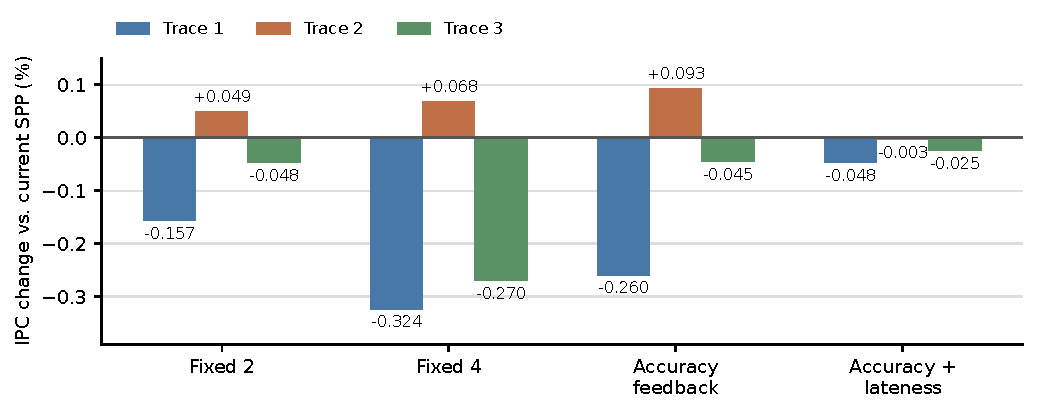
\includegraphics[width=0.92\linewidth]{figures/task1/distance_ipc.pdf}
\caption{IPC change from current SPP for each distance policy.}
\end{figure}

\begin{figure}[htbp]
\centering
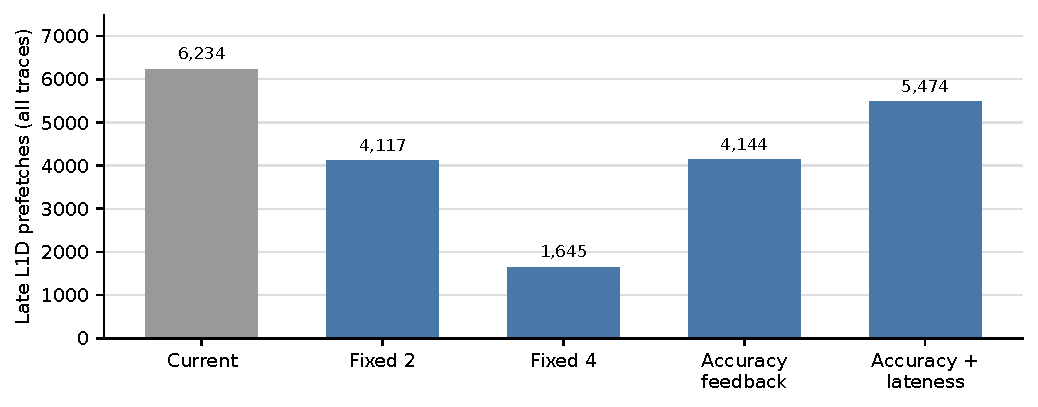
\includegraphics[width=0.92\linewidth]{figures/task1/distance_late.pdf}
\caption{Late L1D prefetches across the three traces. Fewer late requests did not always mean higher IPC.}
\end{figure}
\FloatBarrier

\section{Storage overhead}

The following table counts the fields actually declared in the current
code. The IP only needs 8 bits because of the mask. The software valid
bit uses a one-byte \texttt{bool}; it is not packed into a single bit.

\begin{table}[htbp]
\centering
\small
\begin{tabular}{lrrr}
\toprule
Field & Number of values & Bits per value & Bits per entry \\
\midrule
\texttt{valid} & 1 & 8 & 8 \\
\texttt{ip} & 1 & 8 & 8 \\
\texttt{last\_cl\_addr} & 1 & 64 & 64 \\
\texttt{stride\_array} & 16 & 64 & 1,024 \\
\texttt{curr\_index} & 1 & 8 & 8 \\
\texttt{size} & 1 & 8 & 8 \\
\texttt{last\_stride} & 1 & 64 & 64 \\
\texttt{num\_iterations} & 1 & 16 & 16 \\
\texttt{confidence} & 1 & 8 & 8 \\
\texttt{non\_uniform\_confidence} & 1 & 8 & 8 \\
\texttt{lru} & 1 & 32 & 32 \\
\midrule
Total field payload & & & 1,248 \\
\bottomrule
\end{tabular}
\caption{Stored bits in one SPP tracker.}
\end{table}

One tracker has 1,248 bits, or 156 bytes, of fields. The 24 trackers
therefore have 29,952 bits, or 3,744 bytes, of field payload. GCC 7 adds
12 bytes of alignment padding per tracker, making
\texttt{sizeof(IP\_TRACKER)} equal to 168 bytes. The actual tracker
array occupies 4,032 bytes.

The accuracy controller adds two 64-bit snapshots and one 8-bit degree
limit. This is another 136 bits, or 17 bytes. The total field payload
is therefore 30,088 bits, or 3,761 bytes. Counting tracker padding, the
sum of the object sizes is 4,049 bytes, or 32,392 bits. This does not
include executable code, temporary stack variables, or gaps that the
linker might leave between globals.

The ChampSim prefetch counters already exist, so they do not add new
SPP-only storage. The 16 signed 64-bit strides take most of the space.
The distance experiments are not active, so their extra variables are
not included in this total.

\clearpage
\part{Task 2: Instruction-Conscious L2 Replacement}

 Task 2A implements a static
Instruction-Conscious RRIP (I-RRIP) L2 replacement policy that gives
instruction lines priority over data lines. Task 2B makes it dynamic,
using set dueling to switch between I-RRIP and SRRIP. Both are compared
with LRU and SRRIP on the three traces.



\section{Task 2A: Static I-RRIP}

\subsection{Exposing Instruction Information to L2 Replacement}
In ChampSim, replacement policies do not receive packet type details in \texttt{update\_replacement\_state}. We need this for the purposes of differentiating instruction and data accesses. We updated the interface across \texttt{inc/cache.h}, \texttt{src/cache.cc} and \texttt{src/ooo\_cpu.cc}, and the replacement policy files to pass \texttt{uint8\_t} \texttt{isInstruction} (taken from \texttt{packet.instruction}). This allows the replacement to distinguish instruction accesses from data accesses during insertion and promotion. The condition for this check also includes checking if the packet is issued as a load or a prefetch because instruction fetches are always loads.

\subsection{Policy Design: Insertion, Promotion, and Eviction}
Standard SRRIP uses a 2-bit RRPV counter per cache block, where 0 represents MRU and 3 represents use that was long ago. Our implementation in \texttt{irrip.l2c\_repl} modifies all three components:

\subsubsection{Insertion Policy}
\begin{itemize}
    \item \textbf{Instruction blocks:} Inserted at $\text{RRPV} = 2$ ($maxRRPV-1$).
    \item \textbf{Data blocks:} Inserted at $\text{RRPV} = 3$ ($\text{maxRRPV}$).
\end{itemize}
Data accesses in server workloads to be single-use. Inserting data blocks directly at $\text{RRPV} = 3$ allows dead data to be evicted on the very next miss in that set without aging resident instruction blocks. If a data block has genuine temporal reuse, its first hit will promote it to $\text{RRPV} = 1$, giving it more chance that it will stay in the cache. We had tested another policy wherein data blocks were inserted at 2 and instruction blocks at 1, but this caused a slowdown (this is the iRRIP old).

\subsubsection{Promotion Policy (Hits)}
\begin{itemize}
    \item \textbf{Instruction hit:} Promoted to $\text{RRPV} = 0$.
    \item \textbf{Data hit:} Promoted to $\text{RRPV} = 1$.
\end{itemize}
In an earlier test policy (\texttt{irrip\_moderate}), both instruction and data hits were promoted to 0. This again caused a slowdown, probably because these data lines started to stick around the cache for longer when in reality they gave no benefit. As far as data hits are concerned though, we also had tested another policy wherein the lines were gradually promoted (decrement by 1 each time until it hits 0), but this again caused a slowdown, implying very less reuse of data. Finally, we settled on promoting data hits to 1 and instruction hits to 0, which gave the best performance.

\subsubsection{Eviction (Victim Selection)}
When looking for a replacement victim:
\begin{enumerate}
    \item First check for any block at $\text{RRPV} = 3$ that is a data block (\texttt{block.instruction == 0}). If found, evict it.
    \item If no data block is at $\text{RRPV} = 3$, select any block at $\text{RRPV} = 3$ (these are going to be instruction lines).
    \item If no block has $\text{RRPV} = 3$, increment the RRPV of all blocks in the set and repeat.
\end{enumerate}
Checking for data victims first at $\text{maxRRPV}$ gives aged instruction lines an extra chance of staying in cache if there is any data block ready for eviction. This is the same for all three policies (iRRIP-new, iRRIP-Moderate, and iRRIP-Old).

\subsection{Results and Discussion}
Table~\ref{tab:results-2a} and Figure~\ref{fig:results-2a} show the comparison between LRU, SRRIP, iRRIP-Moderate, iRRIP-Old, and our static iRRIP policy.

\begin{table}[H]
\centering
\small
\caption{Task 2A Performance Metrics (25M warmup + 25M simulation instructions).}
\label{tab:results-2a}
\resizebox{\linewidth}{!}{%
\begin{tabular}{llrrrrrrr}
\toprule
\textbf{Trace} & \textbf{Policy} & \textbf{IPC} & \textbf{Speedup} & \textbf{L2C Load} & \textbf{L2C Instr} & \textbf{L2C Data} & \textbf{Norm. L2C} & \textbf{L2C Red.} \\
 & & & \textbf{vs LRU} & \textbf{MPKI} & \textbf{MPKI} & \textbf{MPKI} & \textbf{Load MPKI} & \textbf{vs LRU (\%)} \\
\midrule
Trace 1 & LRU            & 0.2318 & 1.0000 & 17.745 & 10.389 & 7.356 & 1.0000 & 0.00\% \\
Trace 1 & SRRIP          & 0.2318 & 0.9998 & 17.664 & 10.581 & 7.083 & 0.9954 & +0.46\% \\
Trace 1 & iRRIP-Moderate & 0.2318 & 0.9999 & 17.550 & 10.032 & 7.517 & 0.9890 & +1.10\% \\
Trace 1 & iRRIP-Old      & 0.2319 & 1.0001 & 17.689 & 9.744 & 7.944 & 0.9968 & +0.32\% \\
Trace 1 & \textbf{iRRIP} & \textbf{0.2323} & \textbf{1.0020} & 18.281 & \textbf{9.346} & 8.935 & 1.0302 & -3.02\% \\
\midrule
Trace 2 & LRU            & 0.2503 & 1.0000 & 28.164 & 19.626 & 8.538 & 1.0000 & 0.00\% \\
Trace 2 & SRRIP          & 0.2513 & 1.0039 & 26.419 & 18.460 & 7.959 & 0.9381 & +6.19\% \\
Trace 2 & iRRIP-Moderate & 0.2546 & 1.0171 & 23.978 & 15.136 & 8.842 & 0.8514 & +14.86\% \\
Trace 2 & iRRIP-Old      & 0.2566 & 1.0250 & 21.918 & 12.754 & 9.163 & 0.7782 & +22.18\% \\
Trace 2 & \textbf{iRRIP} & \textbf{0.2593} & \textbf{1.0357} & \textbf{20.957} & \textbf{10.531} & 10.427 & \textbf{0.7441} & \textbf{+25.59\%} \\
\midrule
Trace 3 & LRU            & 0.3818 & 1.0000 & 3.949 & 1.119 & 2.831 & 1.0000 & 0.00\% \\
Trace 3 & SRRIP          & 0.3815 & 0.9992 & 4.033 & 1.192 & 2.842 & 1.0212 & -2.12\% \\
Trace 3 & iRRIP-Moderate & 0.3817 & 0.9998 & 3.943 & 1.069 & 2.873 & 0.9983 & +0.17\% \\
Trace 3 & iRRIP-Old      & 0.3820 & 1.0005 & 3.818 & 0.949 & 2.869 & 0.9668 & +3.32\% \\
Trace 3 & \textbf{iRRIP} & \textbf{0.3823} & \textbf{1.0012} & 3.951 & \textbf{0.849} & 3.101 & 1.0003 & -0.03\% \\
\bottomrule
\end{tabular}%
}
\end{table}

\begin{figure}[H]
\centering
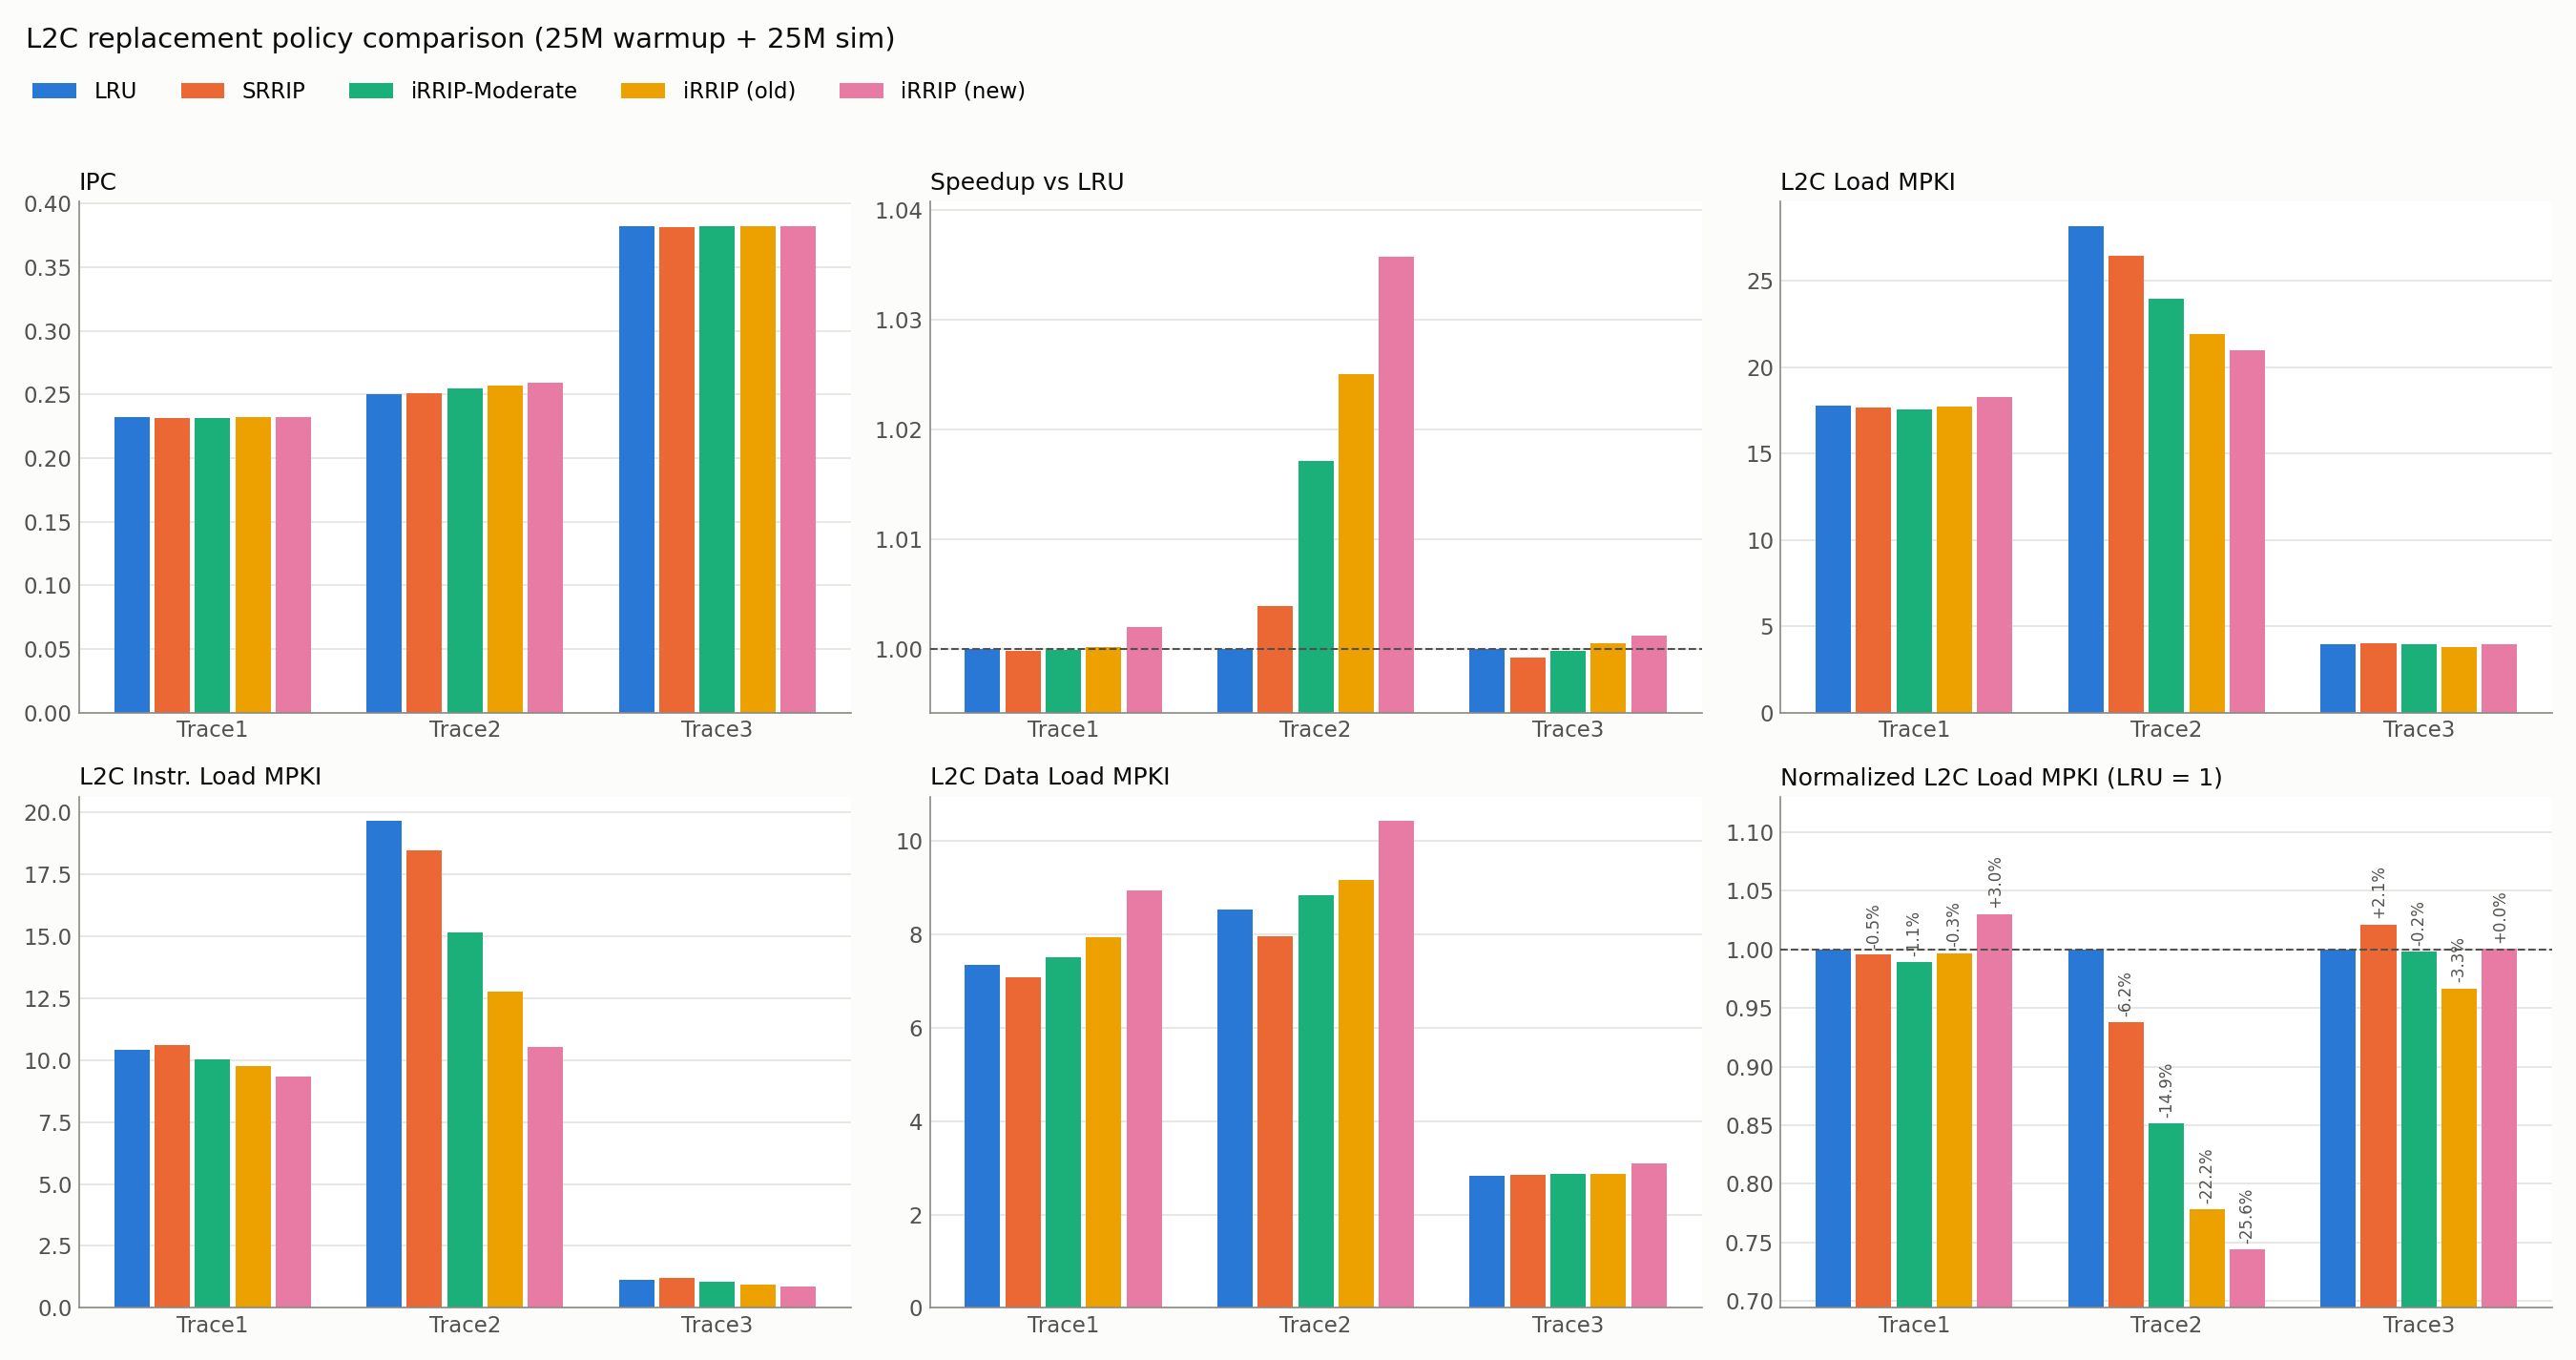
\includegraphics[width=0.98\linewidth]{figures/task2a/policy_comparison_all.png}
\caption{Task 2A Results: Comparison of LRU, SRRIP, iRRIP-Moderate, iRRIP-Old, and iRRIP across IPC, Speedup, and MPKI metrics.}
\label{fig:results-2a}
\end{figure}

\begin{figure}[H]
\centering
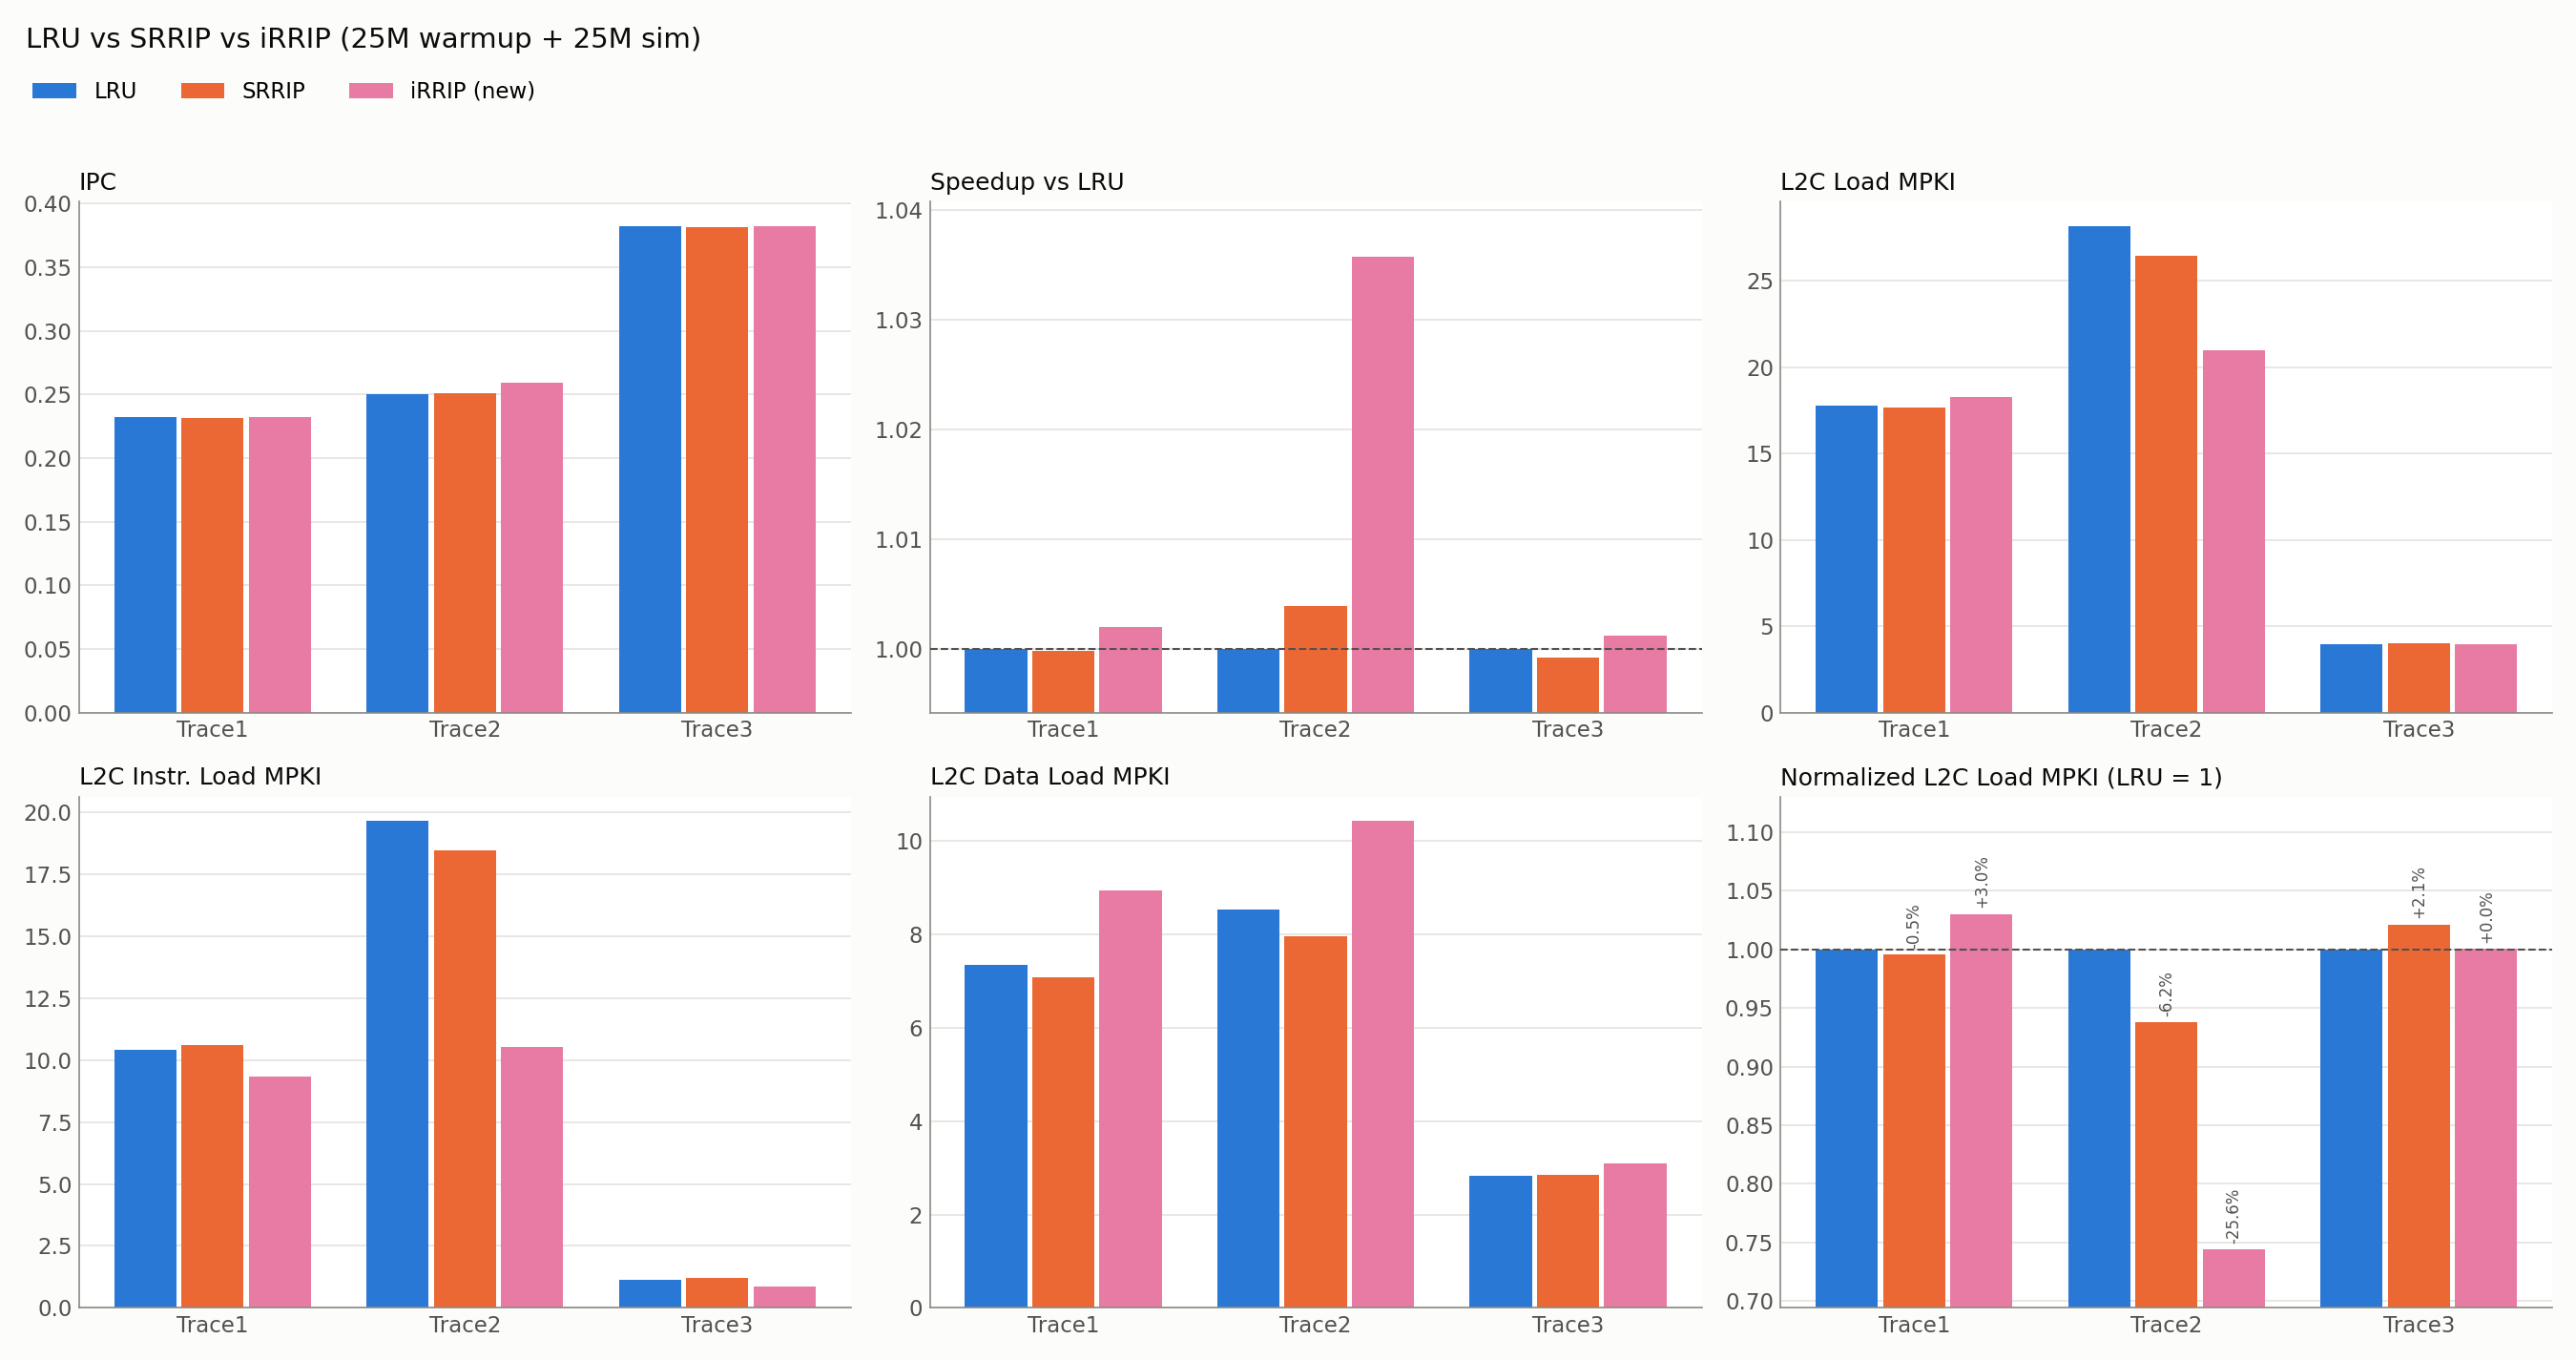
\includegraphics[width=0.98\linewidth]{figures/task2a/policy_comparison_final.png}
\caption{Task 2A Results: Final comparison of LRU, SRRIP, and iRRIP across IPC, Speedup, and MPKI metrics.}
\label{fig:results-2a-final}
\end{figure}

On Trace 2, which has a large instruction footprint, static iRRIP increases IPC from 0.2503 to 0.2593 (\textbf{+3.57\% speedup}), ahead of iRRIP-Old (+2.50\%) and iRRIP-Moderate (+1.71\%). Total L2C Load MPKI decreases by \textbf{25.59\%} (from 28.16 down to 20.96), and instruction MPKI drops by nearly half (\textbf{46.34\% reduction}, from 19.63 to 10.53). On Traces 1 and 3, instruction MPKI also drops by 10.0\% and 24.1\% without hurting overall IPC (+0.20\% and +0.12\% speedup, the highest of all policies on both traces).

\section{Task 2B: Dynamic I-RRIP}

\subsection{Motivation}
Statically deprioritizing data works well for workloads like Trace 2 where instruction misses dominate. However, during execution phases where instruction working sets fit comfortably in cache, prioritizing instructions could increase data misses. A dynamic policy monitors workload behavior and switches between iRRIP and standard SRRIP.

\subsection{Leader Sets}
We implement set dueling using 16 dedicated leader sets out of 1024 total L2 sets:
\begin{itemize}
    \item Leader sets are chosen with a uniform stride of 64: $\text{is\_leader}(set) \iff (set \pmod{64} == 0)$ to ensure these sets are distributed across the cache and not clustered in one region.
    \item Dedicating 16 sets uses $16 / 1024 = 1.5625\%$ of cache capacity, which provides a representative sample of working set behavior across the cache with minimal capacity loss on follower sets.
    \item We ran all the thresholds with different numbers of leader sets (8, 16, 32, 64). 16 leader sets (1.6\% of the L2C) keeps the leader-set overhead negligible. 16 also gives the widest stable threshold range (0.20--0.35). Moreover, it has higher speedups compared to 32 and 64 leader sets. 8 leader sets would be noisier, even if the average speedup is marginally better. Hence, 16 is the best choice here. Average speed was obtained by taking the geometric mean of speedups across all three traces since these are ratios.

\end{itemize}

\subsection{Decision Policy and History Decay}
Leader sets always run standard SRRIP to monitor unskewed cache pressure.
\begin{itemize}
    \item \textbf{Decision Ratio:} We track instruction accesses, instruction misses, total accesses, and total misses on the leader sets. Every 4,096 accesses (\texttt{DECISION\_INTERVAL}), we evaluate:
    \begin{equation}
    \text{Ratio} = \frac{\text{leader\_instr\_acc} + \text{leader\_instr\_miss}}{\text{leader\_total\_acc} + \text{leader\_total\_miss}}
    \end{equation}
    If $\text{Ratio} > \text{INSTR\_THRESH}$, follower sets switch to iRRIP mode; otherwise, they use SRRIP.
    \item \textbf{History Decay:} At the end of every interval, all counters are decayed by 10\%:
    $$\text{counter} \leftarrow \lfloor \text{counter} \times 0.9 \rfloor$$
    Decaying history ensures the policy adapts to workload phase changes rather than remaining stuck on past access patterns. 
\end{itemize}

\subsection{Threshold Sensitivity Study}
We evaluated 7 threshold values ($\theta \in \{0.20, 0.25, 0.30, 0.35, 0.40, 0.45, 0.50\}$) with 16 leader sets. Table~\ref{tab:results-2b} and Figure~\ref{fig:summary-2b} show the results.

\begin{table}[H]
\centering
\small
\caption{Task 2B Dynamic I-RRIP Sensitivity across 7 Values of $\theta$.}
\label{tab:results-2b}
\resizebox{\linewidth}{!}{%
\begin{tabular}{llrrrrrrr}
\toprule
\textbf{Trace} & \textbf{Policy / Threshold} & \textbf{IPC} & \textbf{Speedup} & \textbf{L2C Instr} & \textbf{L2C Data} & \textbf{L2C Load} & \textbf{Instr. Red.} & \textbf{Data Red.} \\
 & & & \textbf{vs LRU} & \textbf{MPKI} & \textbf{MPKI} & \textbf{MPKI} & \textbf{vs LRU (\%)} & \textbf{vs LRU (\%)} \\
\midrule
Trace 1 & SRRIP                  & 0.2318 & 0.9998 & 10.581 & 7.083 & 17.664 & -1.85\% & +3.71\% \\
Trace 1 & Static iRRIP           & 0.2323 & 1.0020 & 9.346 & 8.935 & 18.281 & +10.04\% & -21.46\% \\
Trace 1 & dyn\_iRRIP ($\theta=0.20$) & 0.2324 & 1.0023 & 9.361 & 8.890 & 18.251 & +9.90\% & -20.85\% \\
Trace 1 & dyn\_iRRIP ($\theta=0.25$) & 0.2324 & 1.0023 & 9.361 & 8.890 & 18.251 & +9.90\% & -20.85\% \\
Trace 1 & dyn\_iRRIP ($\theta=0.30$) & 0.2324 & 1.0023 & 9.361 & 8.890 & 18.251 & +9.90\% & -20.85\% \\
Trace 1 & \textbf{dyn\_iRRIP ($\theta=0.35$)} & \textbf{0.2324} & \textbf{1.0023} & \textbf{9.357} & \textbf{8.885} & \textbf{18.242} & \textbf{+9.94\%} & \textbf{-20.78\%} \\
Trace 1 & dyn\_iRRIP ($\theta=0.40$) & 0.2318 & 0.9998 & 10.581 & 7.083 & 17.664 & -1.85\% & +3.71\% \\
Trace 1 & dyn\_iRRIP ($\theta=0.45$) & 0.2318 & 0.9998 & 10.581 & 7.083 & 17.664 & -1.85\% & +3.71\% \\
Trace 1 & dyn\_iRRIP ($\theta=0.50$) & 0.2318 & 0.9998 & 10.581 & 7.083 & 17.664 & -1.85\% & +3.71\% \\
\midrule
Trace 2 & SRRIP                  & 0.2513 & 1.0039 & 18.460 & 7.959 & 26.419 & +5.94\% & +6.79\% \\
Trace 2 & Static iRRIP           & 0.2593 & 1.0357 & 10.531 & 10.427 & 20.957 & +46.34\% & -22.12\% \\
Trace 2 & dyn\_iRRIP ($\theta=0.20$) & 0.2592 & 1.0356 & 10.581 & 10.390 & 20.971 & +46.08\% & -21.69\% \\
Trace 2 & dyn\_iRRIP ($\theta=0.25$) & 0.2592 & 1.0356 & 10.581 & 10.390 & 20.971 & +46.08\% & -21.69\% \\
Trace 2 & dyn\_iRRIP ($\theta=0.30$) & 0.2592 & 1.0356 & 10.581 & 10.390 & 20.971 & +46.08\% & -21.69\% \\
Trace 2 & \textbf{dyn\_iRRIP ($\theta=0.35$)} & \textbf{0.2592} & \textbf{1.0356} & \textbf{10.581} & \textbf{10.390} & \textbf{20.971} & \textbf{+46.08\%} & \textbf{-21.69\%} \\
Trace 2 & dyn\_iRRIP ($\theta=0.40$) & 0.2572 & 1.0273 & 12.723 & 9.651 & 22.374 & +35.17\% & -13.04\% \\
Trace 2 & dyn\_iRRIP ($\theta=0.45$) & 0.2558 & 1.0220 & 14.034 & 9.295 & 23.329 & +28.49\% & -8.86\% \\
Trace 2 & dyn\_iRRIP ($\theta=0.50$) & 0.2517 & 1.0053 & 18.086 & 8.143 & 26.228 & +7.85\% & +4.63\% \\
\midrule
Trace 3 & SRRIP                  & 0.3815 & 0.9992 & 1.192 & 2.842 & 4.033 & -6.54\% & -0.38\% \\
Trace 3 & Static iRRIP           & 0.3823 & 1.0012 & 0.849 & 3.101 & 3.951 & +24.06\% & -9.54\% \\
Trace 3 & dyn\_iRRIP ($\theta=0.20$) & 0.3823 & 1.0012 & 0.851 & 3.088 & 3.939 & +23.91\% & -9.09\% \\
Trace 3 & dyn\_iRRIP ($\theta=0.25$) & 0.3823 & 1.0012 & 0.851 & 3.088 & 3.939 & +23.91\% & -9.09\% \\
Trace 3 & dyn\_iRRIP ($\theta=0.30$) & 0.3823 & 1.0012 & 0.851 & 3.088 & 3.939 & +23.91\% & -9.09\% \\
Trace 3 & \textbf{dyn\_iRRIP ($\theta=0.35$)} & \textbf{0.3823} & \textbf{1.0012} & \textbf{0.849} & \textbf{3.086} & \textbf{3.935} & \textbf{+24.11\%} & \textbf{-9.02\%} \\
Trace 3 & dyn\_iRRIP ($\theta=0.40$) & 0.3815 & 0.9992 & 1.192 & 2.842 & 4.033 & -6.54\% & -0.38\% \\
Trace 3 & dyn\_iRRIP ($\theta=0.45$) & 0.3815 & 0.9992 & 1.192 & 2.842 & 4.033 & -6.54\% & -0.38\% \\
Trace 3 & dyn\_iRRIP ($\theta=0.50$) & 0.3815 & 0.9992 & 1.192 & 2.842 & 4.033 & -6.54\% & -0.38\% \\
\bottomrule
\end{tabular}%
}
\end{table}

\begin{figure}[H]
\centering
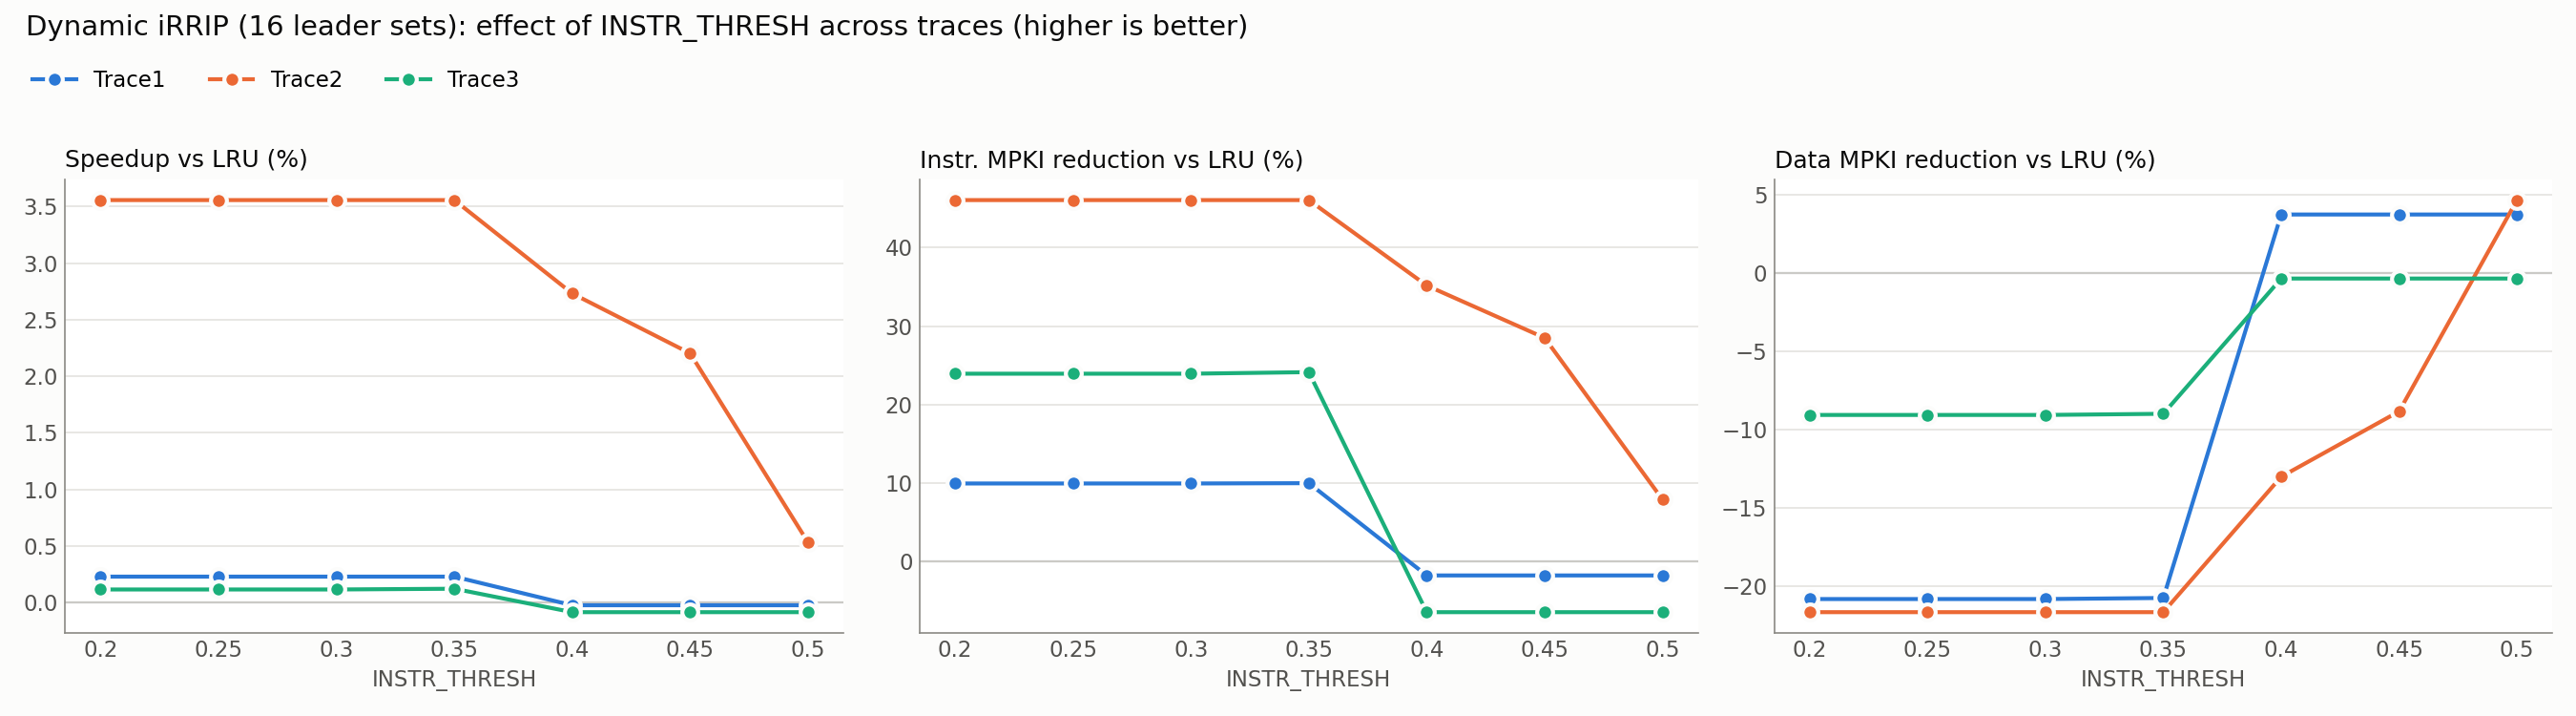
\includegraphics[width=0.98\linewidth]{figures/task2b/summary_vs_threshold.png}
\caption{Task 2B Sensitivity: Impact of \texttt{INSTR\_THRESH} on Speedup, Instruction MPKI, and Data MPKI across all three traces (16 leader sets).}
\label{fig:summary-2b}
\end{figure}

Figures~\ref{fig:speedup-2b}--\ref{fig:load-2b} show each metric separately for every trace, with static iRRIP (dashed) and SRRIP (dotted) as reference lines. For $\theta \le 0.35$, dynamic iRRIP sits on the static iRRIP line. For $\theta \ge 0.40$, it falls onto the SRRIP line on Traces 1 and 3. On Trace 2 it moves gradually between the two.

\begin{figure}[H]
\centering
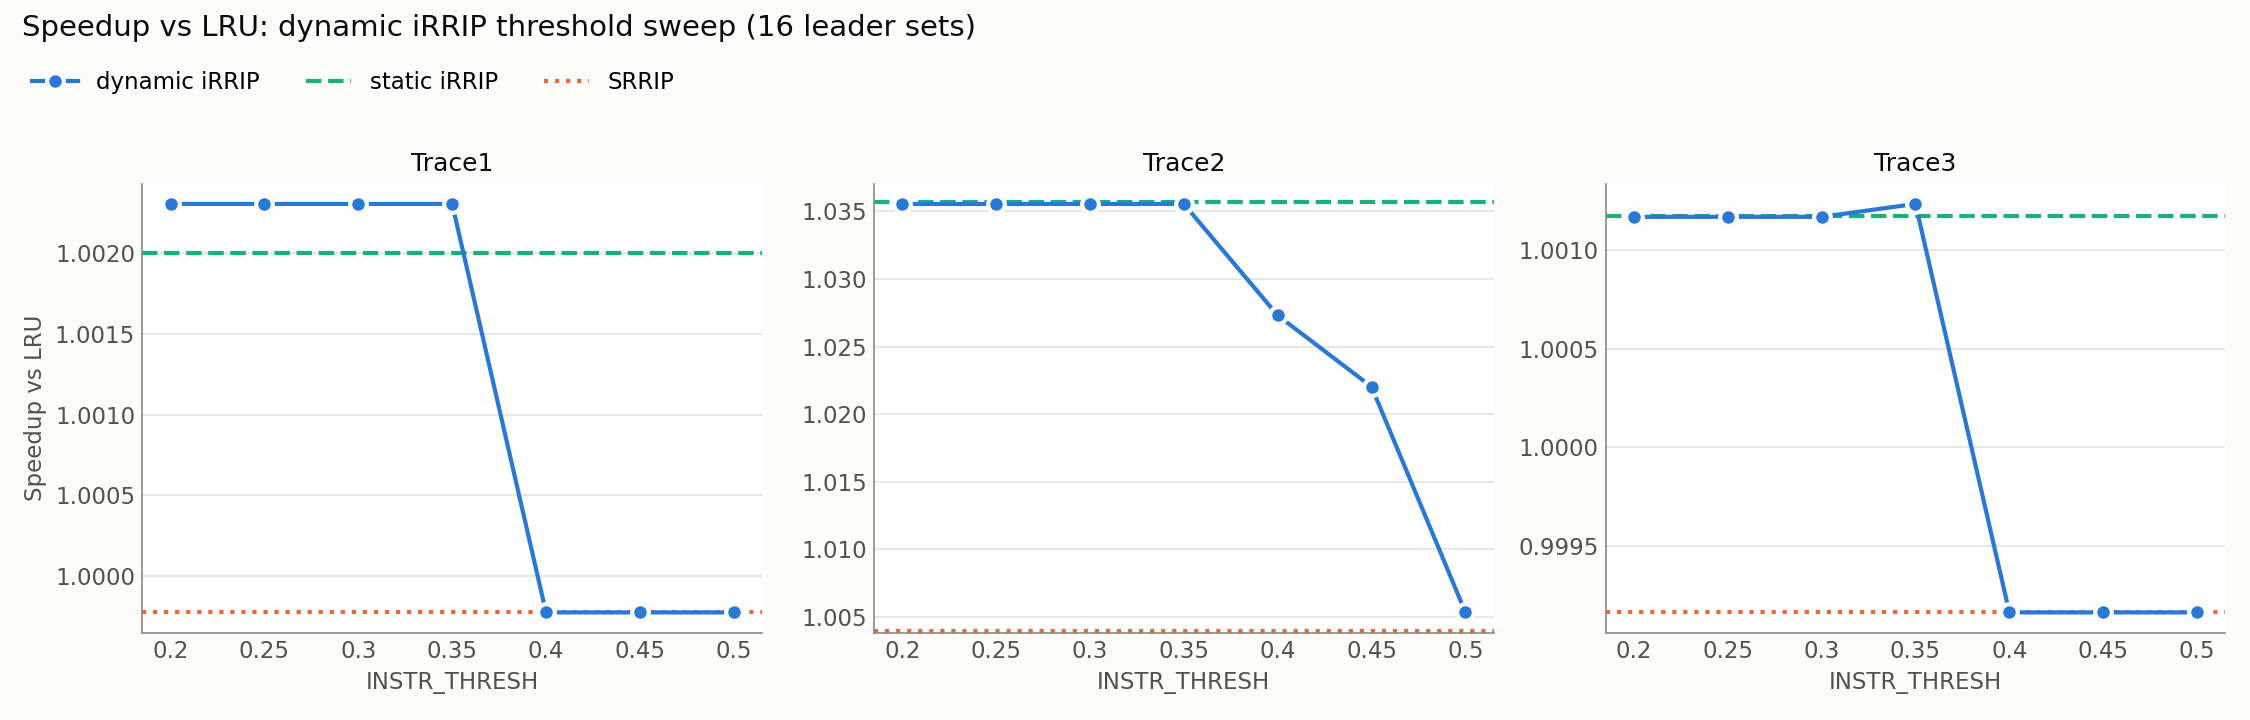
\includegraphics[width=0.98\linewidth]{figures/task2b/speedup_vs_threshold.png}
\caption{Task 2B: Speedup vs LRU across \texttt{INSTR\_THRESH} values, compared with static iRRIP and SRRIP. On Trace 1, dynamic iRRIP is slightly above static iRRIP for $\theta \le 0.35$.}
\label{fig:speedup-2b}
\end{figure}

\begin{figure}[H]
\centering
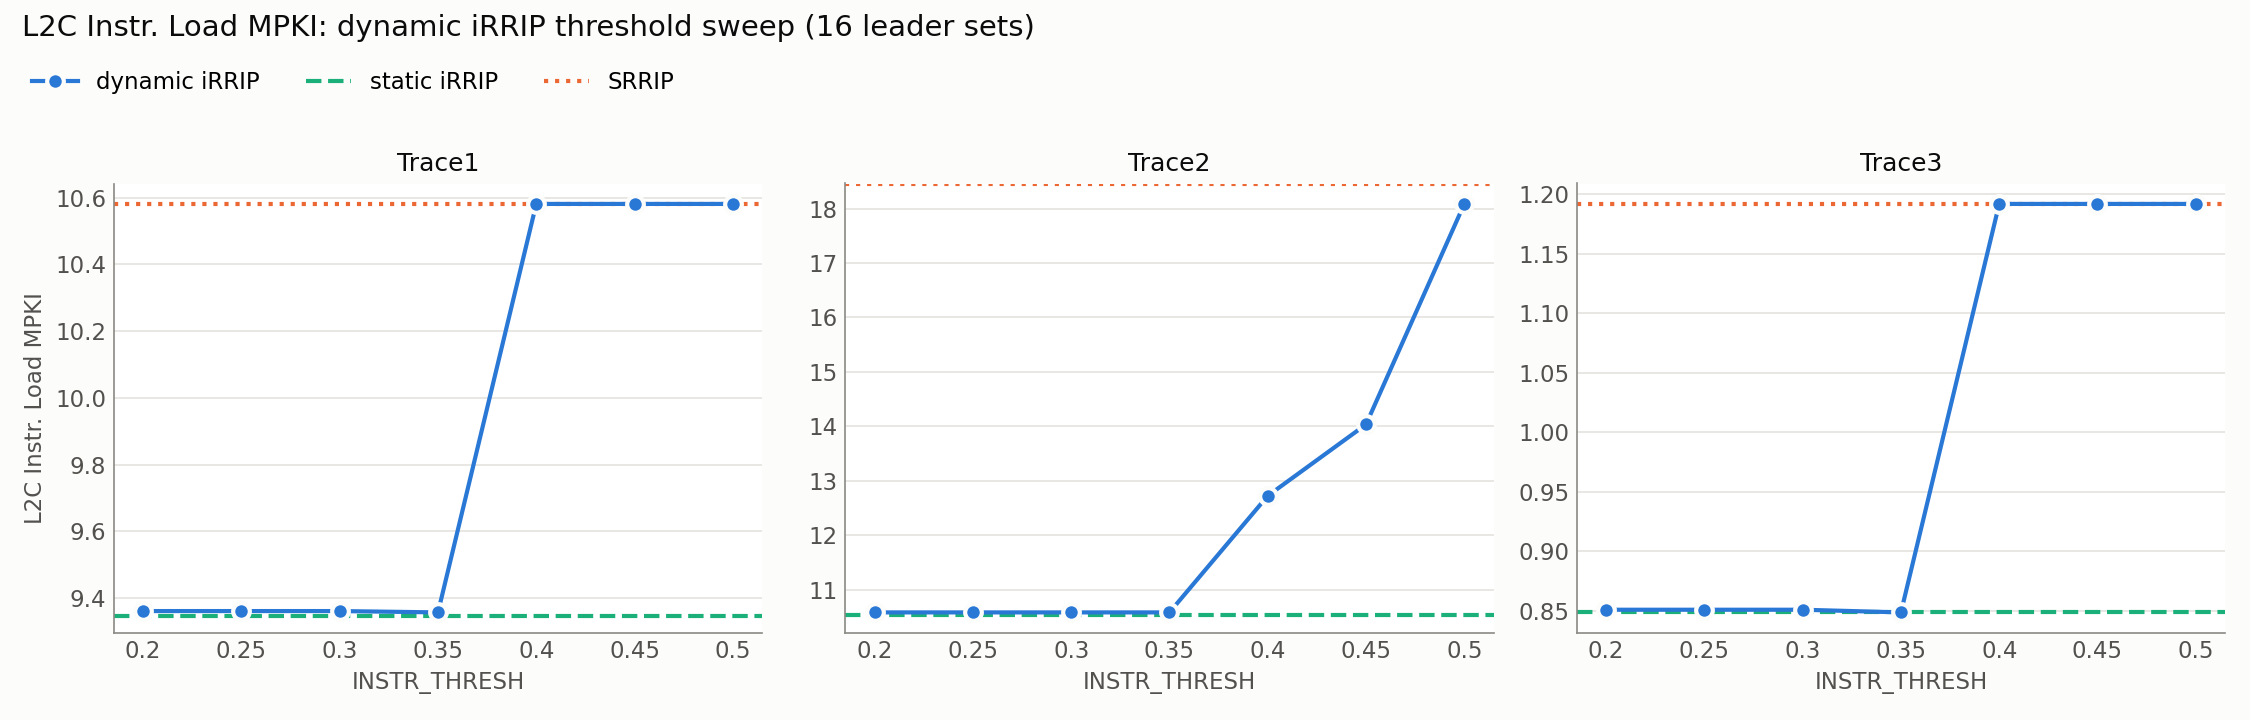
\includegraphics[width=0.98\linewidth]{figures/task2b/instr_mpki_vs_threshold.png}
\caption{Task 2B: L2C Instruction Load MPKI across \texttt{INSTR\_THRESH} values. Instruction MPKI stays at the static iRRIP level up to $\theta = 0.35$ and rises towards SRRIP after that.}
\label{fig:instr-2b}
\end{figure}

\begin{figure}[H]
\centering
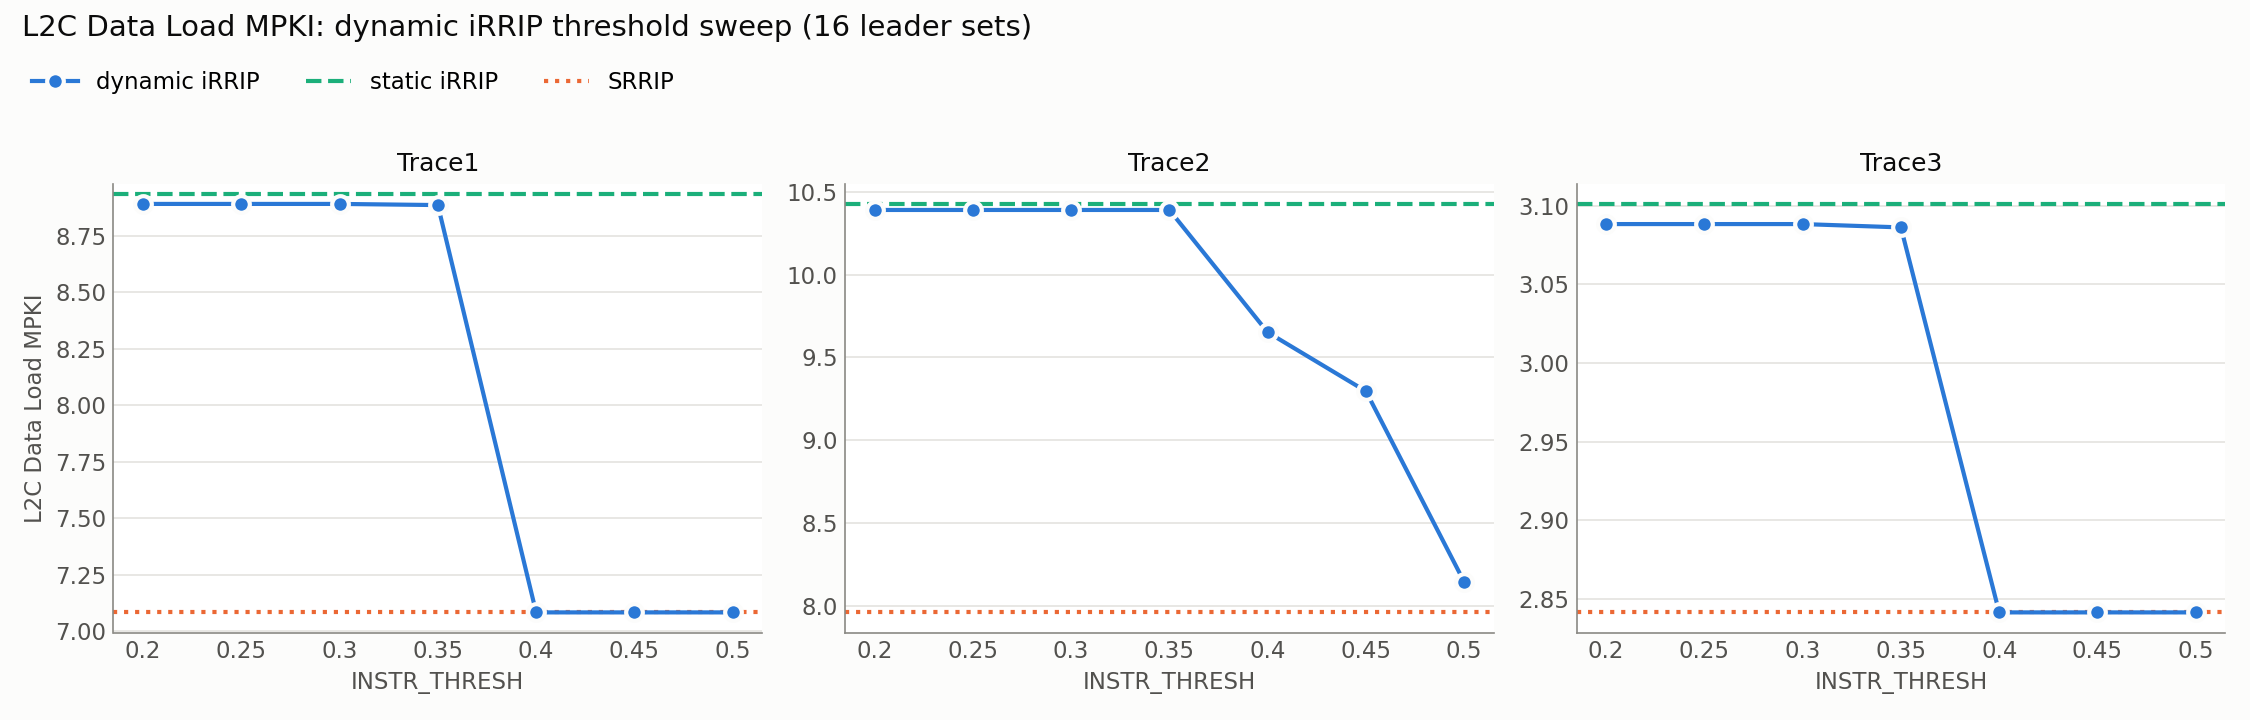
\includegraphics[width=0.98\linewidth]{figures/task2b/data_mpki_vs_threshold.png}
\caption{Task 2B: L2C Data Load MPKI across \texttt{INSTR\_THRESH} values. Data MPKI is the mirror image of instruction MPKI: it is highest while iRRIP is active and drops to the SRRIP level once the policy falls back.}
\label{fig:data-2b}
\end{figure}

\begin{figure}[H]
\centering
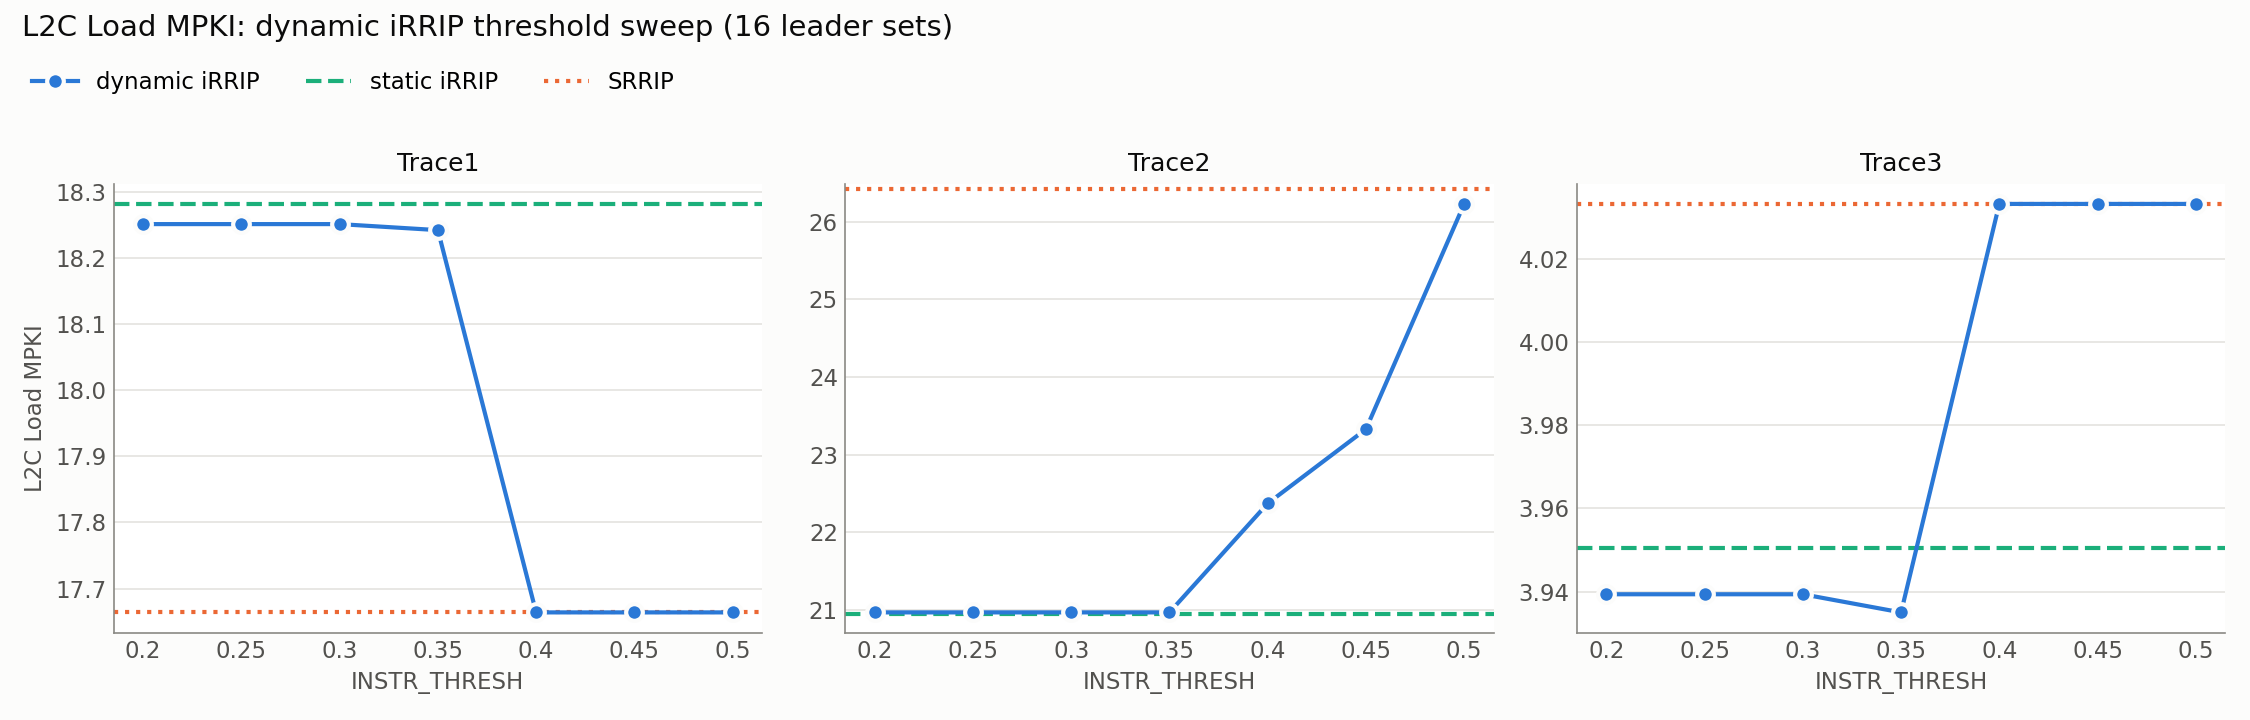
\includegraphics[width=0.98\linewidth]{figures/task2b/load_mpki_vs_threshold.png}
\caption{Task 2B: Total L2C Load MPKI across \texttt{INSTR\_THRESH} values. On Trace 2, total misses rise steeply above $\theta = 0.35$. On Traces 1 and 3, the total changes little because fewer instruction misses are offset by more data misses.}
\label{fig:load-2b}
\end{figure}

\begin{figure}[H]
\centering
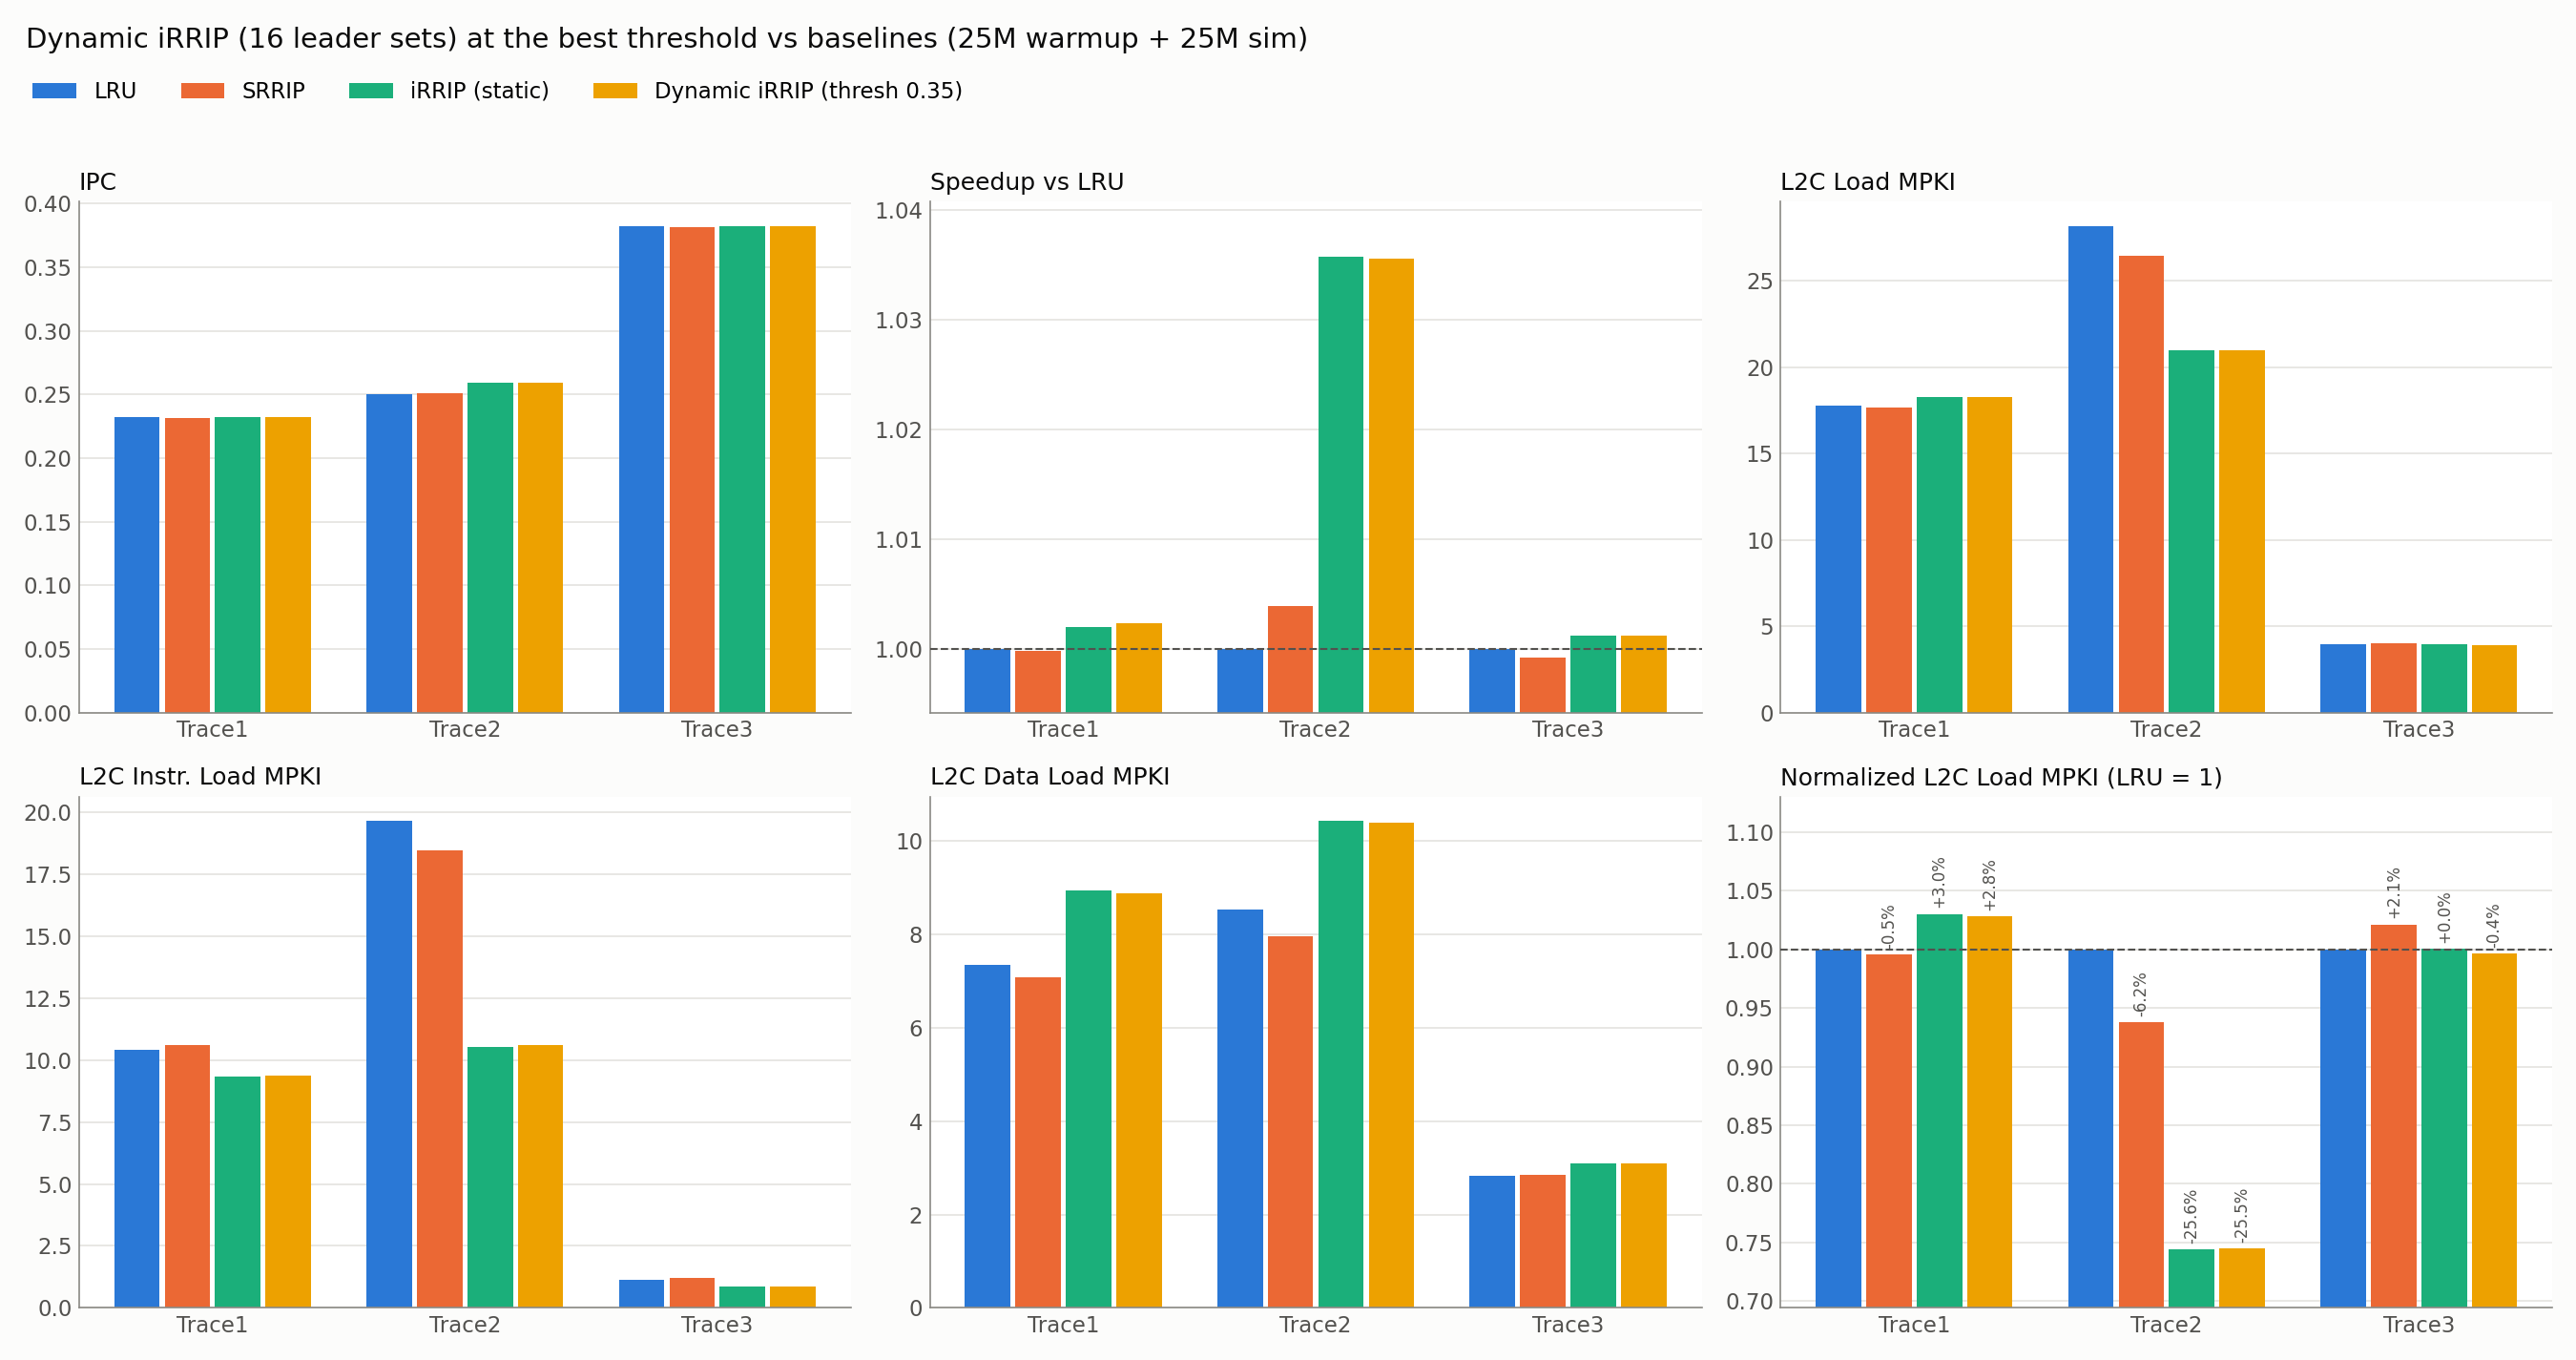
\includegraphics[width=0.98\linewidth]{figures/task2b/dynamic_irrip_comparison.png}
\caption{Task 2B Results: Dynamic iRRIP at the chosen threshold ($\theta = 0.35$) compared with LRU, SRRIP, and static iRRIP across IPC, Speedup, and MPKI metrics.}
\label{fig:results-2b}
\end{figure}

\subsection{Analysis of Threshold Choices}
The sensitivity sweep shows two distinct regions:
\begin{enumerate}
    \item \textbf{Active iRRIP Region ($\theta \le 0.35$):} The leader-set ratio stays above the threshold for practically the whole run, so the follower sets use iRRIP and the results are nearly identical for $\theta = 0.20$ to $0.35$. They also closely track static iRRIP: on Trace 2 the speedup is +3.56\% (static: +3.57\%) and instruction MPKI drops by 46.1\% (from 19.63 to 10.58); on Traces 1 and 3 the speedups are +0.23\% and +0.12\%, with instruction MPKI reductions of about 10\% and 24\%.
    \item \textbf{SRRIP Fallback Region ($\theta \ge 0.40$):} On Traces 1 and 3 the ratio never crosses 0.40, so the policy behaves exactly like SRRIP (identical IPC and MPKI). It loses the instruction MPKI benefit and runs slightly slower than LRU ($-0.02\%$ and $-0.08\%$). On Trace 2 the ratio crosses the threshold only during part of the execution, so the policy switches between the two modes and the benefit fades gradually: speedup falls from +2.73\% ($\theta = 0.40$) to +2.20\% (0.45) and +0.53\% (0.50), and the instruction MPKI reduction falls from 35.2\% to 7.9\%. Data MPKI recovers in exchange (from $-13.0\%$ to $+4.6\%$ vs LRU), but this does not make up for the extra instruction misses.
    \item \textbf{Chosen Threshold ($\theta = 0.35$):} All thresholds in $[0.20, 0.35]$ give the best IPC on every trace. Within this range, 0.35 is marginally the best: it has the highest IPC on Trace 3 and the lowest L2C Load MPKI on Traces 1 and 3. Since it is also the most conservative value in the stable region, it is the first to fall back to SRRIP when instruction pressure drops. We therefore choose $\theta = 0.35$ (Figure~\ref{fig:results-2b}).
\end{enumerate}

\section{Conclusion}
By filtering dead data on insertion ($\text{RRPV} = 3$), enforcing tiered MRU promotion (giving instructions priority at $\text{RRPV} = 0$), and prioritizing data victims during eviction, the instruction-conscious policies significantly improve frontend throughput. On the code-heavy Trace 2 workload, static iRRIP achieves a \textbf{+3.57\% speedup} and cuts instruction MPKI by \textbf{46.34\%}. The dynamic policy with 16 leader sets and $\theta = 0.35$ matches this, with a \textbf{+3.56\% speedup} and a \textbf{46.08\%} instruction MPKI reduction on Trace 2. It is also slightly ahead on Trace 1 (+0.23\% vs +0.20\%), and it can fall back to SRRIP when instruction pressure is low.

\clearpage
\part{Task 3: SPP with Prefetch-Aware Dynamic I-RRIP}

Task 3 combines the Task 1 SPP at L1D with
the Task 2B Dynamic I-RRIP at L2, modified to be prefetch-aware. It is
compared with no-prefetch LRU, standalone SPP, and Dynamic I-RRIP on the
three traces, using 25M warmup and 25M simulation instructions.


\begin{table}[H]
\centering\small
\caption{Evaluated configurations.}
\begin{tabularx}{\linewidth}{lXX}
\toprule
Configuration & L1D prefetcher & L2 replacement \\
\midrule
Baseline & None & LRU \\
Standalone SPP & Task 1 SPP & LRU \\
Dynamic I-RRIP & None & Task 2B Dynamic I-RRIP \\
Task 3 & Task 1 SPP & Prefetch-aware Dynamic I-RRIP \\
\bottomrule
\end{tabularx}
\end{table}

Task 3 and the Task 2B comparison both use 16 leader sets, a decision
interval of 4096 leader accesses, threshold 0.35, and history decay 0.9.

\section{Task 3: Prefetch-Aware Dynamic I-RRIP}

Each cache line has a two-bit RRPV between 0 and 3. Lines at 0 receive
the most protection, while lines at 3 can be evicted. If no line is at 3,
we increase the RRPVs in the set until a victim is available.
Table 2 lists the insertion and hit updates for both replacement modes.

\begin{table}[H]
\centering\small
\caption{Task 3 insertion and promotion behavior.}
\begin{tabularx}{\linewidth}{lXX}
\toprule
Event & RRIP mode & I-RRIP mode \\
\midrule
Instruction hit & Set to 0 & Set to 0 \\
Demand-data hit & Set to 0 & Decrement by 1, minimum 0 \\
Data-prefetch hit & Unchanged & Unchanged \\
Writeback hit & Unchanged & Unchanged \\
Instruction fill & Insert at 2 & Insert at 2 \\
Demand-data fill & Insert at 2 & Insert at 3 \\
Data-prefetch fill & Insert at 3 & Insert at 3 \\
Writeback fill & Insert at 3 & Insert at 3 \\
\bottomrule
\end{tabularx}
\end{table}

\subsection{Insertion and Eviction Policy}
We insert data prefetches and writebacks at RRPV 3 in both modes.
A prefetch may be useful later, but inserting it with high priority can
push out a line that is already being reused. Similarly, a writeback from
an upper cache does not necessarily mean the CPU will access that line
again soon. Inserting these lines at 3 makes them easy to replace if they
receive no demand hits.

This choice can also evict a useful prefetch before it is needed. If demand
reaches the line while it is still cached, the hit promotes it according
to the active policy. In I-RRIP mode, we also prefer data lines over
instruction lines when choosing among victims at RRPV 3. Dirty victims
still follow the normal writeback path.

\subsection{Promotion Policy}
We leave RRPV unchanged on prefetch and writeback hits. A repeated
prefetch should not keep a line protected simply because the prefetcher
requests it again. Setting RRPV to a fixed value on these hits could also
lower the priority of a line that demand accesses had already promoted.

Demand hits provide the reuse information we want. In RRIP mode, a demand
hit sets RRPV to 0. In I-RRIP mode, instruction hits set it to 0, while
data hits decrease it by one. Repeated data hits therefore move a line
through $3\rightarrow2\rightarrow1\rightarrow0$, where it remains on
further hits.

\subsection{Dynamic Selection and Leader Sets}
We use the leader sets to estimate instruction pressure:
\[
\frac{\text{instruction accesses}+\text{instruction misses}}
{\text{all eligible accesses}+\text{all eligible misses}}.
\]
At each decision interval, this ratio determines whether follower sets
use I-RRIP or RRIP. Writebacks are excluded from the counters; prefetch
and translation accesses are included. The interval is counted in leader
updates.

One difference from Task 2B is that Task 3's leader sets also use the
prefetch-aware RRIP updates. Task 2B's leaders use the original RRIP policy.

\section{Results and Discussion}

Tables~\ref{tab:performance} and~\ref{tab:mpki} summarize performance and
cache misses across the three traces. Speedup and coverage use the
no-prefetch LRU baseline.

\begin{table}[H]
\centering\small
\caption{Task 3 performance. Speedup and coverage use no-prefetch LRU.}
\label{tab:performance}
\begin{tabular}{lrrrr}
\toprule
Trace & IPC & Speedup & Accuracy (\%) & Coverage (\%) \\
\midrule
Trace 1 & 0.235501 & 1.013584 & 48.414530 & 7.059000 \\
Trace 2 & 0.263644 & 1.049714 & 35.494400 & 0.715620 \\
Trace 3 & 0.386766 & 1.012307 & 22.060735 & 5.620196 \\
\bottomrule
\end{tabular}

\end{table}

\begin{table}[H]
\centering\small
\caption{Task 3 load misses per 1000 measured instructions.}
\label{tab:mpki}
\begin{tabular}{lrrrr}
\toprule
Trace & L1D load & L2C load & L2 instruction & L2 data \\
\midrule
Trace 1 & 9.924240 & 17.600600 & 9.072720 & 8.527880 \\
Trace 2 & 13.441039 & 18.713359 & 8.316800 & 10.396600 \\
Trace 3 & 3.212160 & 3.493800 & 0.782240 & 2.711560 \\
\bottomrule
\end{tabular}

\end{table}

\subsection{Comparison with Standalone Policies}
All configurations use the same warmup and simulation lengths. Table~\ref{tab:ipc} shows
absolute IPC; Table~\ref{tab:gains} shows the direct Task 3 gains.

\begin{table}[H]
\centering\small
\caption{IPC of the four configurations on each trace.}
\label{tab:ipc}
\begin{tabular}{lrrr}
\toprule
Configuration & Trace 1 & Trace 2 & Trace 3 \\
\midrule
No prefetch + LRU & 0.232345 & 0.251158 & 0.382065 \\
Standalone SPP & 0.233569 & 0.251236 & 0.383645 \\
Dynamic I-RRIP & 0.232375 & 0.259223 & 0.382297 \\
Task 3 & 0.235501 & 0.263644 & 0.386766 \\
\bottomrule
\end{tabular}

\end{table}

\begin{table}[H]
\centering\small
\caption{Task 3 IPC improvement over the standalone policies.}
\label{tab:gains}
\begin{tabular}{lrr}
\toprule
Trace & vs standalone SPP (\%) & vs Dynamic I-RRIP (\%) \\
\midrule
Trace 1 & +0.827079 & +1.345081 \\
Trace 2 & +4.938909 & +1.705631 \\
Trace 3 & +0.813588 & +1.169005 \\
Geometric mean & +2.174911 & +1.406326 \\
\bottomrule
\end{tabular}

\end{table}

Task 3 has higher IPC than both standalone policies on all three traces.
The largest improvement over standalone SPP is on Trace 2, at 4.94\%.
The gains over Dynamic I-RRIP range from 1.17\% to 1.71\%.
Across all three traces, the geometric-mean improvements are
2.17\% over standalone SPP and 1.41\% over Dynamic I-RRIP.

\subsection{Performance and Prefetching Behavior}
Figure~\ref{fig:performance} shows the IPC and prefetching results.
Trace 2 has the largest speedup over the baseline, at 4.97\%, even though
its L1D miss coverage is only 0.72\%. This is consistent with the benefit
of instruction protection at L2. On Traces 1 and 3, coverage is higher,
at 7.06\% and 5.62\%, respectively. The combined policy improves IPC on
these traces as well, although the gains are smaller than on Trace 2.

\begin{figure}[H]
\centering
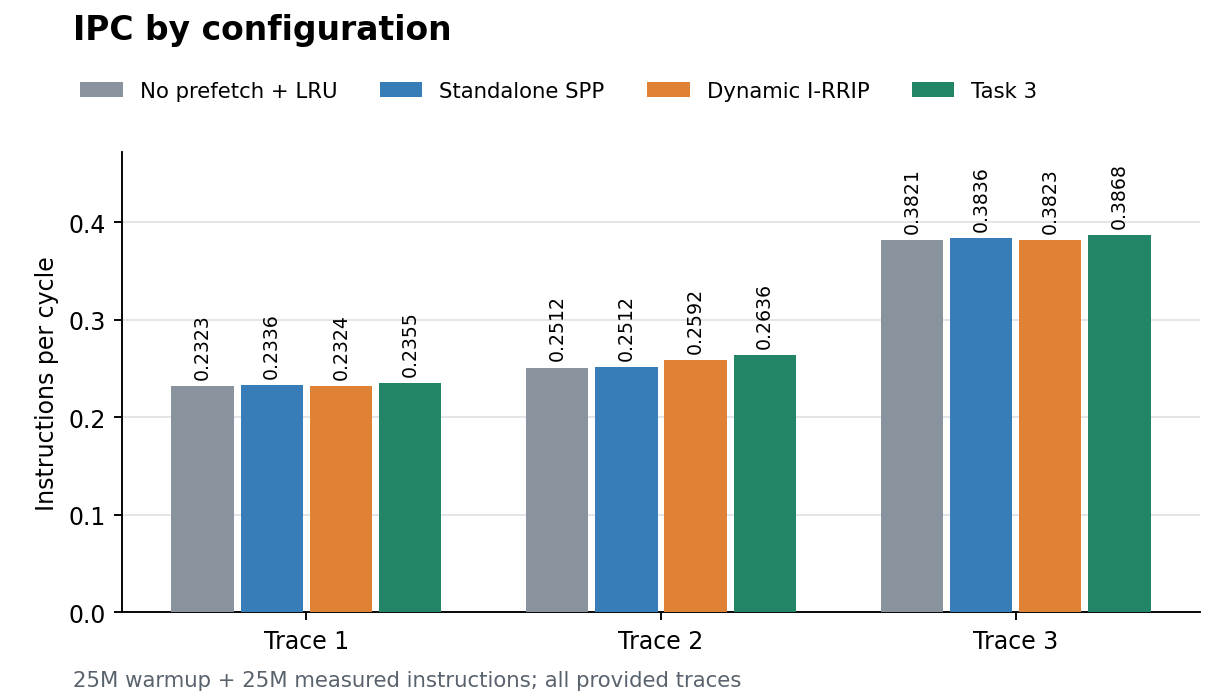
\includegraphics[width=0.48\linewidth]{figures/task3/ipc.png}\hfill
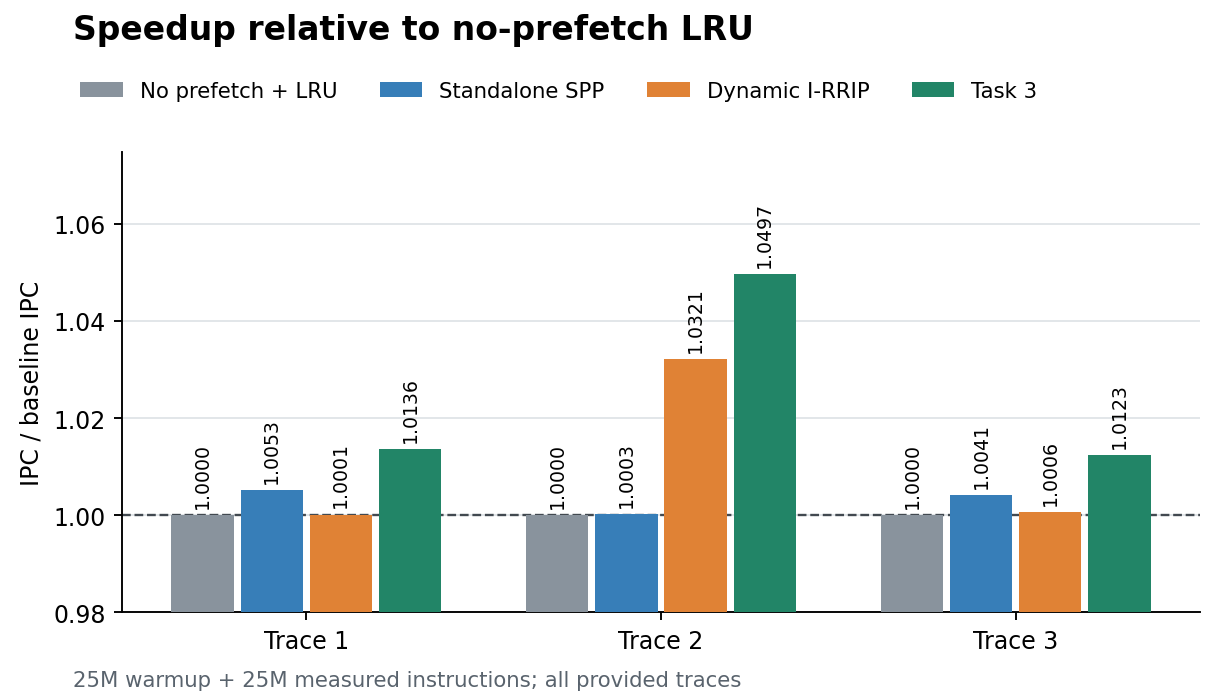
\includegraphics[width=0.48\linewidth]{figures/task3/speedup.png}\\[5pt]
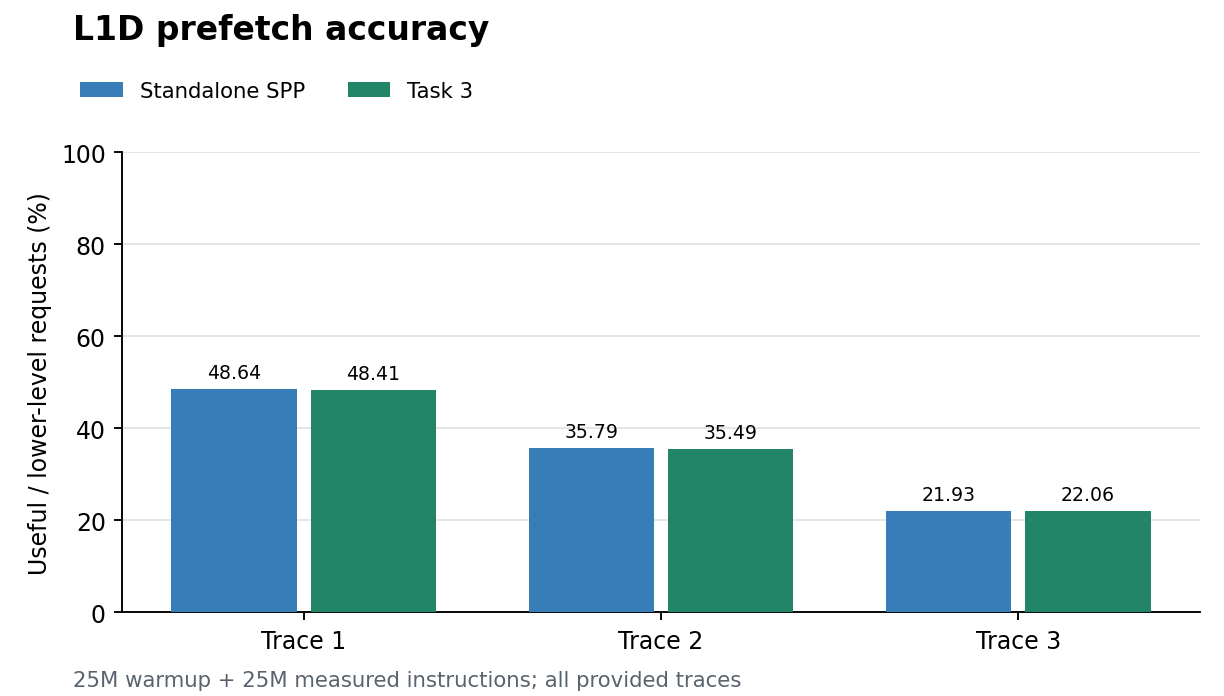
\includegraphics[width=0.48\linewidth]{figures/task3/accuracy.png}\hfill
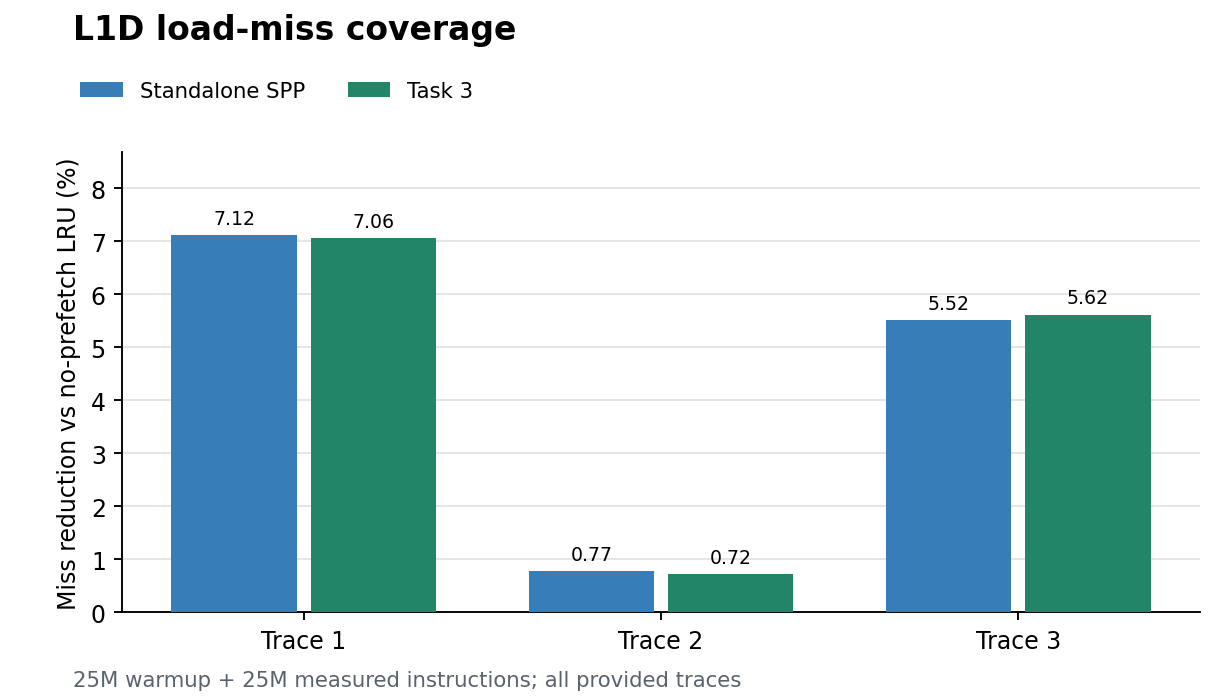
\includegraphics[width=0.48\linewidth]{figures/task3/coverage.png}
\caption{Task 3 performance compared with the baseline and standalone policies.}
\label{fig:performance}
\end{figure}

\newpage
\subsection{Cache Miss Analysis}
Figure~\ref{fig:mpki} shows where the cache misses change. Protecting
instructions can increase data misses, so a lower instruction MPKI does
not always give a lower total L2 MPKI. For example, Task 3 has an L2
instruction MPKI of 8.32 on Trace 2 and a data MPKI of 10.40. Despite this
data-miss cost, it has the highest IPC of the four configurations.
The split helps explain why total MPKI alone is not enough to compare
these policies.

\begin{figure}[H]
\centering
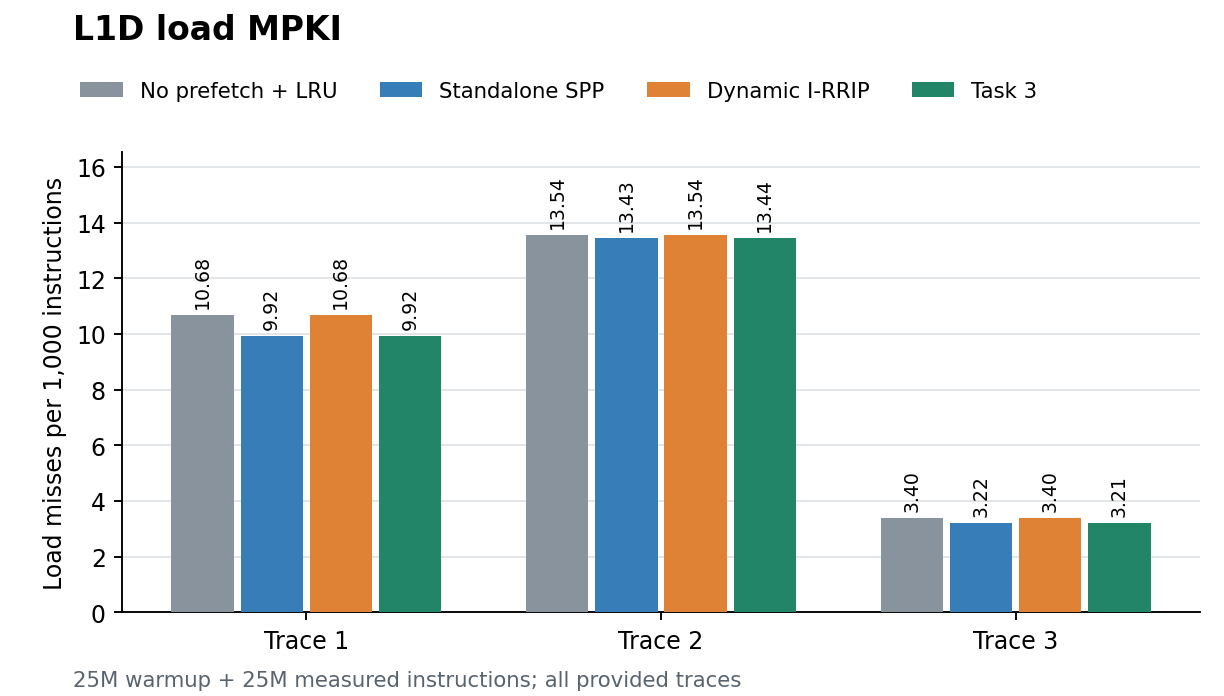
\includegraphics[width=0.48\linewidth]{figures/task3/l1d_load_mpki.png}\hfill
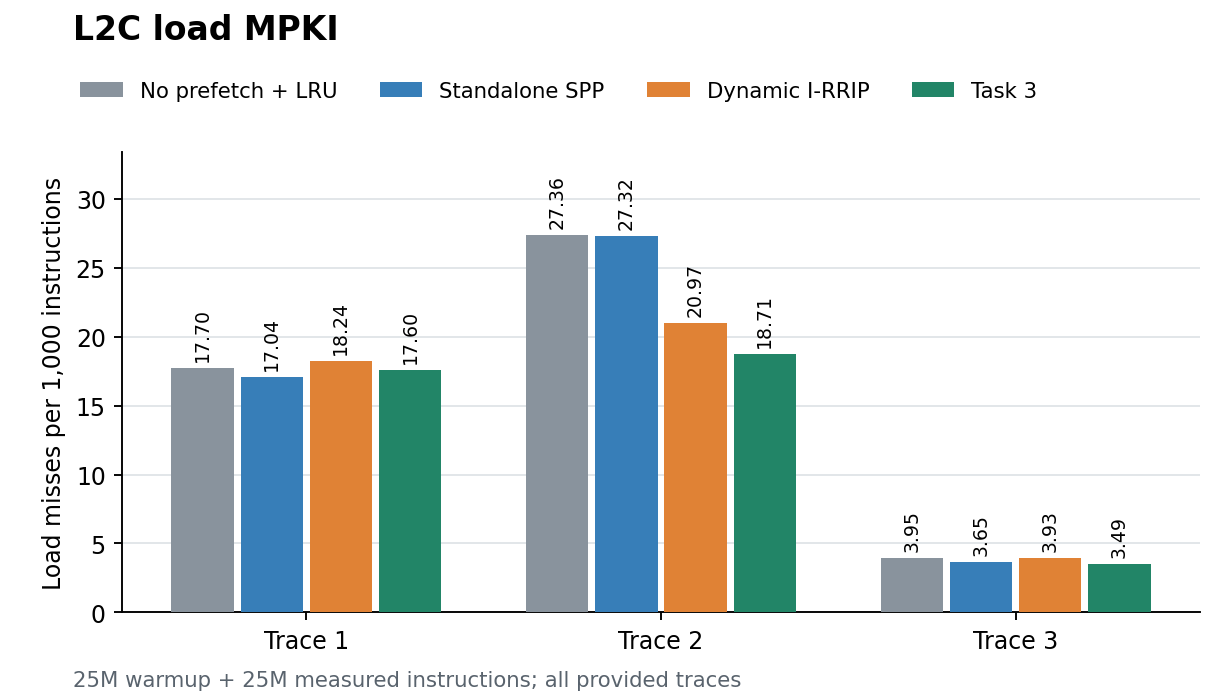
\includegraphics[width=0.48\linewidth]{figures/task3/l2c_load_mpki.png}\\[5pt]
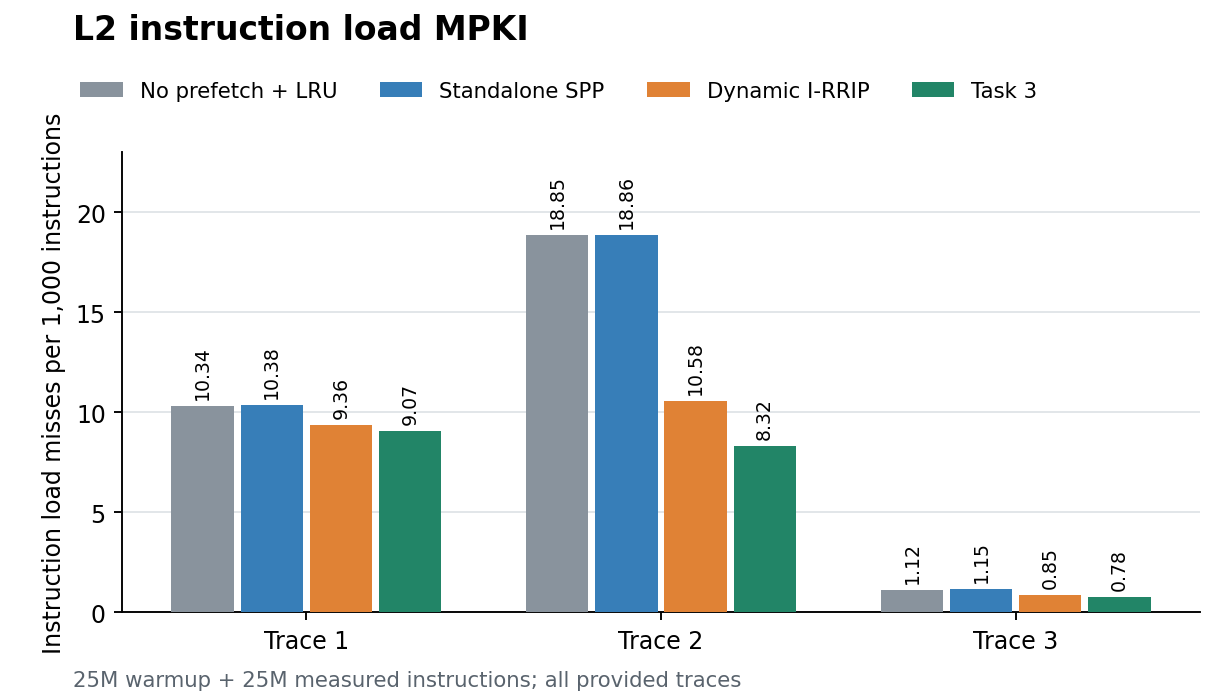
\includegraphics[width=0.48\linewidth]{figures/task3/l2_instruction_load_mpki.png}\hfill
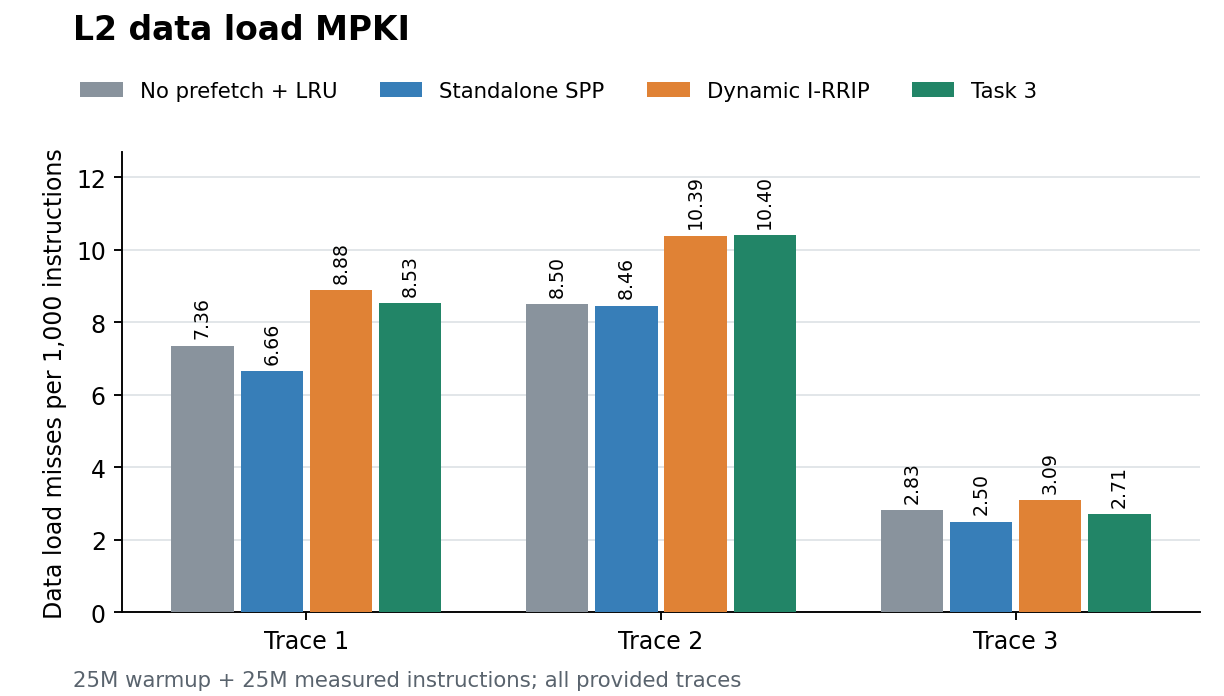
\includegraphics[width=0.48\linewidth]{figures/task3/l2_data_load_mpki.png}
\caption{L1D and L2 load MPKI, with instruction and data misses shown separately.}
\label{fig:mpki}
\end{figure}

\section{Conclusion}
Combining SPP with prefetch-aware Dynamic I-RRIP improves IPC on all
three traces. The geometric-mean gain is \textbf{2.51\% over no-prefetch
LRU}, \textbf{2.17\% over standalone SPP}, and \textbf{1.41\% over
Dynamic I-RRIP}. Trace 2 benefits the most, with a \textbf{4.97\% speedup}
over the baseline. Giving prefetches low insertion priority and promoting
them on demand hits lets us retain the benefit of prefetching while
reducing the protection given to unused data.

\end{document}
